\documentclass[12pt,a4paper,openany]{book} 
\usepackage[typeblock=golden]{stb-titlepage}        

%==== Language setup =================================================
\usepackage[utf8]{inputenc}%...................... Unicode file format

%==== Math setup =====================================================
\usepackage{amsmath}%............................. Advanced math (before fonts)
%\usepackage{amssymb}%............................ AMS Symbol fonts

%==== Font setup (default is Computer Modern) ========================
\usepackage[T1]{fontenc}%......................... Type 1 outline fonts 
\usepackage[bitstream-charter]{mathdesign}%....... Roman+math - Charter
\usepackage{roboto}%.............................. Sans serif - Roboto
\usepackage{textcomp}%............................ Additional text character
\usepackage{bm}%.................................. Bold math symbols (after fonts)

%==== Units and numbers ==============================================
\usepackage{siunitx}%............................. Unit, number and angle output
    \sisetup{detect-all = true, detect-family = true}
    \sisetup{output-decimal-marker = {.} ,
             group-separator = {\,},
             number-unit-product = {\,},
             inter-unit-product = {{\cdot}},
             exponent-product = {{\times}},
             separate-uncertainty = true}
         
%==== Ref's, Bib's and Nomencl =======================================
\usepackage{stb-nomencl}%......................... List of symbols 
    \renewcommand*{\UnitLabel}[1]{~[\,\unit{#1}\,]}
\usepackage{stb-bib}%............................. Bibliography (natbib internally)
    \bibliographystyle{stb-bib-eng-a}
    \renewcommand\bibfont{\small}

%==== Tables + Graphics + Color =====================================
\usepackage{array}%............................... Extended table defs 
    \setlength{\extrarowheight}{2pt}
\usepackage{longtable}%........................... Tables can break over pages
\usepackage{graphicx}%............................ Included graphics
\usepackage[font=small]{caption}%................. Customize captions  
\usepackage[table]{xcolor}%....................... Color setup + colortbl 
    
%==== Extra defs for template ========================================
\makeatletter
%---- TOC entries and case
    \renewcommand\contentsname{Table of contents}
    \renewcommand\listfigurename{List of figures}
    \renewcommand\listtablename{List of tables}
    \renewcommand\bibname{List of references}
    \renewcommand\tableofcontents{\chapter{\contentsname}\@starttoc{toc}}
    \renewcommand\listoffigures{\chapter{\listfigurename}\@starttoc{lof}}
    \renewcommand\listoftables{\chapter{\listtablename}\@starttoc{lot}}
    \renewcommand\bibsection{\chapter{\bibname}}

%---- Plagiarism signatures
    \newcommand\tstrut[1][4ex]{\rule{0pt}{#1}}
    \newcommand\tdots[1][5cm]{\makebox[#1]{\dotfill}}

%---- Summary head line
    \newcommand\sumheading{%
        \rowcolor[gray]{.9}%
        \centering\arraybackslash%
        \bfseries\large}

%==== User Defs ======================================================
%
% Please insert user defined commands here
% and NOT in the document itself!
%
\usepackage{graphicx}
\graphicspath{ {./figs/} }
\usepackage{wrapfig}
\usepackage{array}
\usepackage{multirow}
\usepackage{amsmath}
\usepackage{tabularx}
\usepackage{ragged2e}
\usepackage{microtype}
\usepackage[none]{hyphenat}
\usepackage{xpatch}
\usepackage{tablefootnote}
%
\xpatchcmd{\@makechapterhead}{\vspace*{50\p@}}{\vspace*{5pt}}{\typeout{Success}}{\typeout{Failure!!!}}
%
\makeatother

%==== Title Page =====================================================
\title{\textbf{Design, model and build a USAR robot platform}\\[2ex]
       \large Mechatronic Project 478\\Final Report\\[2ex]}                   
\author{\Large Author: Ronan Wells\\ 
        \large 22961305 \\[5ex]
        \Large Supervisor: Mr. Wayne Swart}                
\address{Department of Mechanical and Mechatronic Engineering\\
        Stellenbosch University \\
        Private Bag X1, Matieland 7602, South Africa.}
\date{2023/03/17}                             

%==== Main Document ==================================================
\setcounter{secnumdepth}{3}
\setcounter{tocdepth}{2}
\raggedbottom
\begin{document}   

\frontmatter%---------------------------------------------------------                    
\maketitle 

\chapter{Plagiarism declaration}

I have read and understand the Stellenbosch University Policy on Plagiarism and the definitions of plagiarism and self-plagiarism contained in the Policy [Plagiarism: The use of the ideas or material of others without acknowledgement, or the re-use of one's own previously evaluated or published material without acknowledgement or indication thereof (self-plagiarism or text-recycling)].

I also understand that direct translations are plagiarism, unless accompanied by an appropriate acknowledgement of the source. I also know that verbatim copy that has not been explicitly indicated as such, is plagiarism.

I know that plagiarism is a punishable offence and may be referred to the University's Central Disciplinary Committee (CDC) who has the authority to expel me for such an offence.

I know that plagiarism is harmful for the academic environment and that it has a negative impact on any profession.

Accordingly all quotations and contributions from any source whatsoever (including the internet) have been cited fully (acknowledged); further, all verbatim copies have been expressly indicated as such (e.g. through quotation marks) and the sources are cited fully.

I declare that, except where a source has been cited, the work contained in this assignment is my own work and that I have not previously (in its entirety or in part) submitted it for grading in this module/assignment or another module/assignment.
I declare that have not allowed, and will not allow, anyone to use my work (in paper, graphics, electronic, verbal or any other format) with the intention of passing it off as his/her own work.

I know that a mark of zero may be awarded to assignments with plagiarism and also that no opportunity be given to submit an improved assignment. 
\vspace{1.5cm}

\noindent
\begin{tabular}{@{}lllll@{}}
\tstrut Signature: &\tdots&	           &            \\
\tstrut Name:      &\tdots& Student no:&\tdots[3cm] \\
\tstrut Date:      &\tdots&            &            \\
\end{tabular}
		

\chapter{Executive summary}

\noindent
\begin{longtable}{|p{\dimexpr \linewidth-2\tabcolsep-2\arrayrulewidth}|}
\hline%------------------------------------------------------------
\sumheading  Title of Project \\
\hline%------------------------------------------------------------
 Design, model and build a USAR robot platform \\
\hline%------------------------------------------------------------
\sumheading  Objectives \\
\hline%------------------------------------------------------------
 Create a model to describe the kinematics of a Load Intuitive Module (LIM). \\
 Build a prototype Urban Search and Rescue (USAR) device which uses LIMs to climb stairs.\\
 Validate the model using the prototype.\\
\hline%------------------------------------------------------------
\sumheading  What is current practice and what are its limitations? \\
\hline%------------------------------------------------------------
 The current practice for USAR platform ranges widely, but the most successful platforms use tracks with paddles for locomotion.
 These devices are effective but very expensive, so there is a need for low cost expendable USAR robots.\\
\hline%------------------------------------------------------------
\sumheading  What is new in this project? \\
\hline%------------------------------------------------------------
 This project will introduce a model to describe a less expensive stair climbing robot platform using LIMs. \\
 
\hline%------------------------------------------------------------
\sumheading  If the project is successful, how will it make a difference? \\
\hline%------------------------------------------------------------
 The model developed in this project can be used to inform future USAR designs. \\

\hline%------------------------------------------------------------
\sumheading  What are the risks to the project being a success? Why is it expected to be successful? \\
\hline%------------------------------------------------------------
 The main risk to this project is that it does not build a working prototype in time. This risk will be mitigated through careful planning and consideration of previous pitfalls.  \\

\hline%------------------------------------------------------------
\sumheading  What contributions have/will other students made/make? \\
\hline%------------------------------------------------------------
 In 2013, Matthew Wilson developed the LIM system as a masters project at the University of Cape Town (UCT).
 Further development on the system was done in final year projects at UCT by students Jordan Haskel, Murray Buchanan, and Richard Daniel Powrie in 2017, 2018, and 2019 respectively.\\
\hline%------------------------------------------------------------
\sumheading  Which aspects of the project will carry on after completion and why? \\
\hline%------------------------------------------------------------
 USAR devices using LIMs as a platform can be designed, built and tested. \\

\hline%------------------------------------------------------------
\sumheading  What arrangements have been/will be made to expedite continuation? \\
\hline%------------------------------------------------------------
 All calculations, designs, and code will be made available to future students. \\

\hline%------------------------------------------------------------
\end{longtable}


%\chapter{Acknowledgments}



\tableofcontents
\listoffigures
\begingroup
\let\clearpage\relax
\listoftables
\endgroup
\let\cleardoublepage\clearpage
%\chapter{List of symbols}
% Use stb-nomenclature + siunitx

\begin{Nomencl}[1cm]
\NomGroup{Constants}%-----------------------------------------------
    \item[$g = $] \qty{9.81}{m/s^2}
\NomGroup{Components}%-----------------------------------------------
	\item[1] LIM frame
	\item[2] Central or "sun" gear
	\item[3] Front idler gear
	\item[4] Rear idler gear
	\item[5] Front outer or "planet" gear
	\item[6] Rear outer or "planet" gear
	\item[7] Body of the device, including the motors and the tail
\NomGroup{Variables}%-----------------------------------------------
	\item[$I_n$]
	\UnitLine{Mass moment of inertia of component n, normal and relative to its relevant axis}{kg.m^2}
	\item[$M_{\mathrm{React}n}$]
	\UnitLine{Reaction moment that the ground or step exerts on wheel n}{N.m}
	\item[$m_n$]
	\UnitLine{Mass of component n}{kg}
	\item[$N$]
	\UnitLine{Number of the step on which the front wheel is placed}{~}
	\item[$N_2$]
	\UnitLine{Number of the step on which the tail makes contact}{~}
	\item[$N_{\mathrm{Planet}}$]
	\UnitLine{Number of teeth on the outer gear}{~}
	\item[$N_{\mathrm{Sun}}$]
	\UnitLine{Number of teeth on the central gear}{~}
	\item[$r_n$]
	\UnitLine{Radius of gear n}{rad/s^2}
	\item[$r_w$]
	\UnitLine{Radius of the wheels}{m}
	\item[$s_{7\mathrm{end}y}$]
	\UnitLine{3x1 Position vector of component the end of the tail}{m}
	\item[$T$]
	\UnitLine{Torque exerted by the motor of component 7 on component 2}{N.m}
	\item[$T_\mathrm{Rated-stall}$ ]
	\UnitLine{The motor stalling torque when the rated voltage is applied}{N.m}
	\item[$t$]
	\UnitLine{Time}{s}
	\item[$V_\mathrm{Rated}$ ]
	\UnitLine{The rated motor voltage}{V}
	\item[$V_\mathrm{Terminal}$ ]
	\UnitLine{The voltage across the motor terminals}{V}
	\item[$\theta_n$]
	\UnitLine{Clockwise angle of component n}{rad}
	\item[$\dot{\theta}_{\mathrm{Frame}}$]
	\UnitLine{Angular velocity of the frame}{rad/s}
	\item[$\dot{\theta}_{\mathrm{Planet}}$]         
	\UnitLine{Angular velocity of the outer gear and wheel}{rad/s}
	\item[$\dot{\theta}_{\mathrm{Sun}}$]
	\UnitLine{Angular velocity of the central gear}{rad/s}
	\item[$\dot{\theta_n}$]
	\UnitLine{Clockwise angular velocity of component n}{rad/s}
	\item[$\ddot{\theta_n}$]
	\UnitLine{Clockwise angular acceleration of component n}{rad/s^2}
	\item[$\mu_5$]
	\UnitLine{Static coefficient of friction between the front wheel and the surface it makes contact with}{~}
	\item[$\mu_{\mathrm{tail}}$]
	\UnitLine{Static coefficient of friction between the tail and the surface it makes contact with}{~}
	\item[$\omega$ ]
	\UnitLine{Motor shaft angular velocity}{rad/s}
	\item[$\omega_\mathrm{Rated-no-load}$ ]
	\UnitLine{Motor shaft angular velocity when the rated voltage is applied and the motor is unloaded}{rad/s}
	\item[$\vec{a_n}$]
	\UnitLine{3x1 Acceleration vector of component n}{m/s^2}
	\item[$\vec{F}_{\mathrm{React}n}$]
	\UnitLine{3x1 Force vector the ground or stairs exert on component n}{N}
	\item[$\vec{f_n}$]
	\UnitLine{3x1 Force vector that component n exerts on component 1}{N}
    \item[$\vec{\mathrm{gf}_3}$]
	\UnitLine{3x1 Force vector that gear n exerts on the inner gear that it contacts}{N}
	\item[$\vec{l_n}$]
	\UnitLine{3x1 Displacement vector from the motor axis to component n}{m}
	\item[$\vec{s_n}$]
	\UnitLine{3x1 Position vector of component n}{m}
	\item[$\vec{u}$]
	\UnitLine{3x1 Displacement vector from the motor axis to the point where the tail contacts the step}{m}
	\item[$\vec{v_n}$]
	\UnitLine{3x1 Velocity vector of component n}{m/s}
	\item[$\vec{w_n}$]
	\UnitLine{3x1 Force vector resulting from the weight of component n}{N}
\NomGroup{Subscripts}%----------------------------------------------
    \item[$x$] Component of a Cartesian vector in the x direction
    \item[$y$] Component of a Cartesian vector in the y direction
    \item[$z$] Component of a Cartesian vector in the z direction
\end{Nomencl}
\clearpage
\begin{Nomencl}[1cm]
\NomGroup{Abbreviations}%-----------------------------------------------
\item[DC] Direct Current
\item[FR] Functional Requirement
\item[LIM] Load Intuitive Module
\item[MATLAB] Matrix Laboratory
\item[MDF] Medium Density Fibreboard
\item[PR] Performance Requirement
\item[PWM] Pulse Width Modulation
\item[RPM] Rotations Per Minute
\item[SR] Stakeholder Requirement
\item[UCT] University of Cape Town
\item[USAR] Urban Search And Rescue
\item[WSL] Windows Subsystem for Linux
\end{Nomencl}


\mainmatter%----------------------------------------------------------
\numberwithin{figure}{chapter}
\numberwithin{table}{chapter}

%\chapter{Introduction}

\section{Background}

Starting from the big picture, gradually narrow focus down to this project and where this report fits in.

\section{Objectives}

The objectives of the project (in some cases the objectives of the report). If necessary describe limitations to the scope.

\section{Motivation}

Why this specific project/report is worthwhile.
 \chapter{Literature review}

\section{USAR robots}

\begin{wrapfigure}{r}{0.35\textwidth} %this figure will be at the right
	\centering
	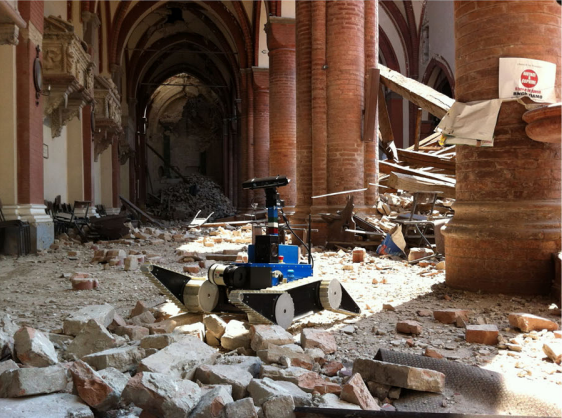
\includegraphics[width=0.35\textwidth]{stateof-tracked}
	\caption{A tracked USAR robot, with paddles for obstacle climbing \citep{stateof}.}
	\label{stateof tracked}
\end{wrapfigure}

In both natural and man-made disasters, USAR operations are critical for reducing casualties. Robots can be deployed in USAR operations to complement human and canine rescuers. Robots have the advantage of being able to be deployed in scenarios too small or too dangerous for humans, and aerial robots such as quadcopters are extremely effective at quickly mapping terrain and providing situational awareness to teams. Other emerging applications of USAR robotics are remote fire fighting, victim interaction, and extraction \citep{stateof}.\\
\begin{wrapfigure}{l}{0.35\textwidth} %this figure will be at the left
	\centering
	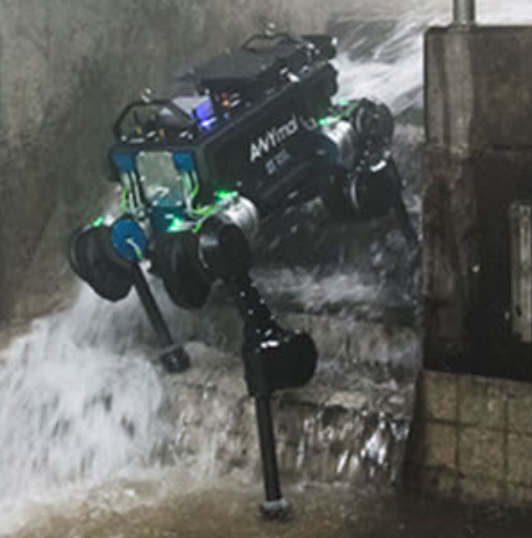
\includegraphics[width=0.35\textwidth]{stateof-wheelleg}
	\caption{ANYmal, a legged USAR robot \citep{stateof}.}
	\label{stateof wheelleg}
\end{wrapfigure}

In order to perform USAR operations, robots need some form of locomotion. For ground robots, this typically involves either tracks, wheels, or legs. \citep{stateof}. Tracked robots with actuated paddles for obstacle climbing, such as the one shown in Figure \ref{stateof tracked}, have been found to perform extremely well. This is evident by their representation in the winners of the Robocup Rescue Robot League (RRL), an event in which teams compete to produce robots for versatile USAR operations \citep{Sheh-2016}. Wheeled robots are generally the simplest and easiest to repair, but can get stuck more easily in uneven terrain. Legged robots provide the advantage of not needing a continuous path, and rapid developments in optical sensors and control systems are enabling them to be even more viable. Wheel-leg hybrid systems will use legged motion for navigating difficult terrain, and wheels when on smooth ground \citep{stateof}. 
\newpage
\section{Load-Intuitive Modules} %~~~~~~~~~~~~~~~~~~~~~~~~~~~~~~~~~~~~~~~~~~~~~~~~~~~~~~~~~~~~~~

\begin{wrapfigure}{r}{0.35\textwidth} %this figure will be at the right
	\centering
	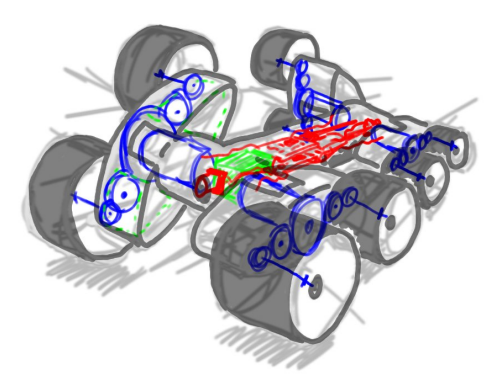
\includegraphics[width=0.35\textwidth]{Wilson-sketch}
	\caption{Systems layout of Wilson's LIM device \citep{Wilson-2013}.}
	\label{Wilson sketch-lit}
\end{wrapfigure}

A Load-Intuitive Module (LIM) refers to a wheel system proposed by Matthew Wilson, shown in Figure \ref{Wilson sketch-lit} \citep{Wilson-2013}. The LIM system uses a two outer "minor wheels" placed on a central hub that can be rotated as a "major wheel". The minor wheels are geared to the central hub such that they drive the vehicle, however if they experience high resistance, for example from hitting an obstacle, the torque will cause the major wheel to rotate instead, flipping one of the minor wheels over the obstacle to automatically climb it. The system is referred to as "Load-Intuitive" because it will intuitively climb over obstacles in response to increased load on the wheels. LIMs are designed to be used in low cost USAR robots, allowing them to climb over objects without the need for many actuators.\\

One advantage LIMs provide over existing locomotion methods is that they can climb obstacles higher than their profile, meaning they can enter low voids while rolling, and climb relatively tall obstacles by flipping over them. Another advantage is that LIMs require minimal actuation, one motor can be used to drive both the rolling and flipping motion, which will reduce costs when compared with other designs.\\

\noindent "LIMed" robot platforms (platforms using LIMs for locomotion) were built individually by four final year students at UCT \citep{Wilson-2013}, \citep{Haskel-2017}, \citep{Buchanan-2018}, and \citep{Powrie-2019}. These platforms show some success in climbing a single step, albeit inconsistently.

\subsection{Wilson's LIM robot} %~~~~~~~~~~~~~~~~~~~~~~~~~~~~~~~~~~~~~~~~~~~~~~~~~~~~~~~~~~~~~~~~~~~~~~~~~~~~~~~~

\begin{wrapfigure}{r}{0.35\textwidth}
	\centering
	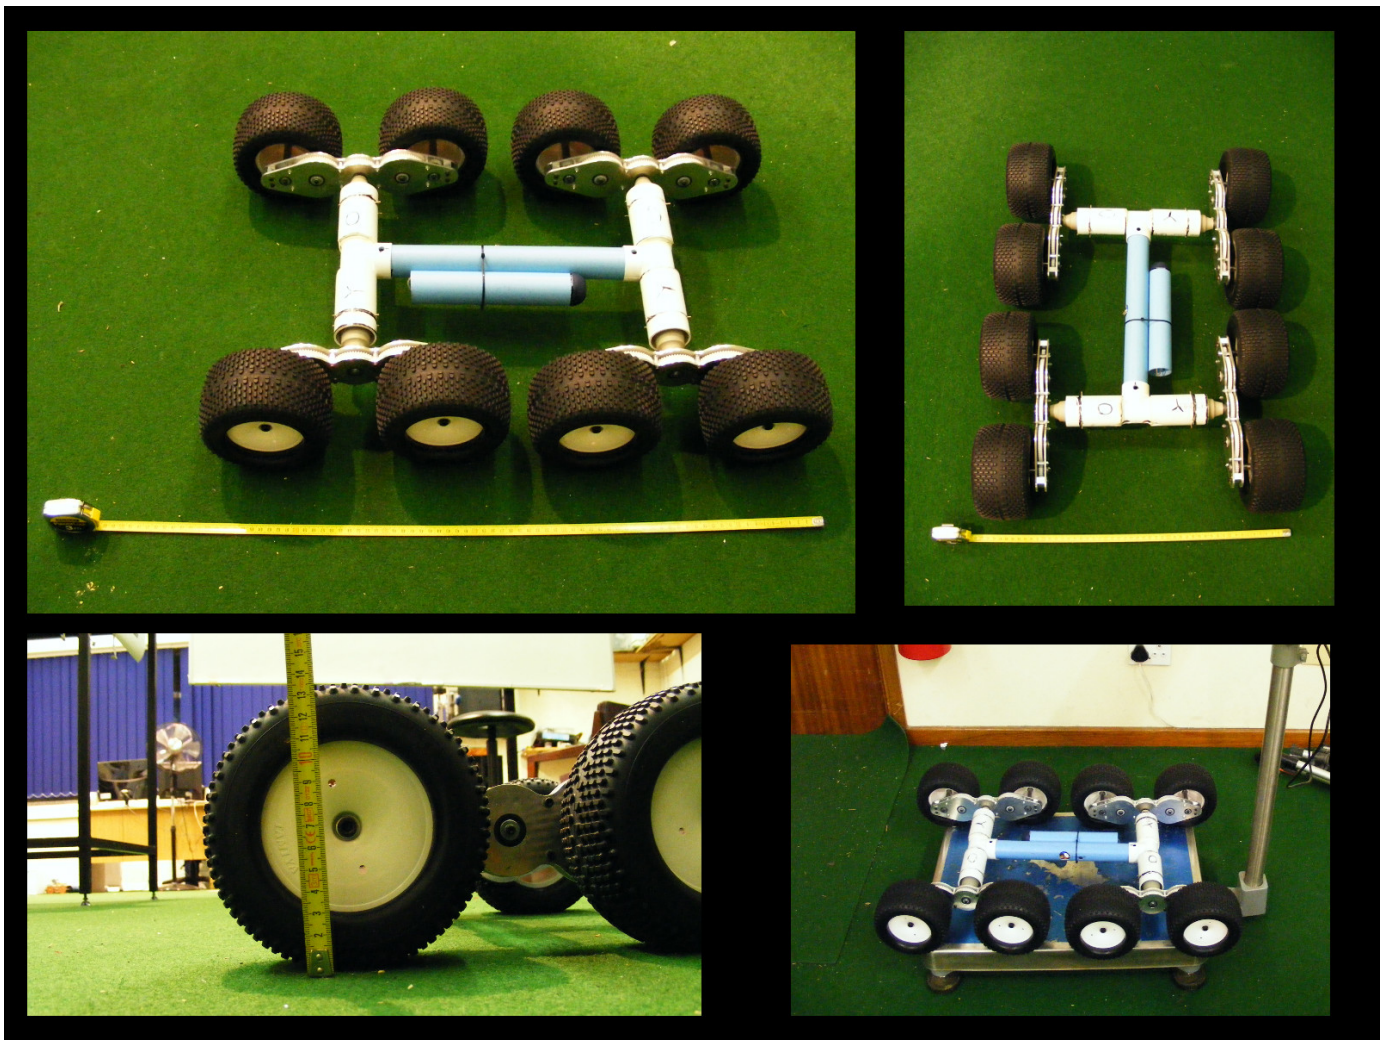
\includegraphics[width=0.35\textwidth]{Wilson-robot}
	\caption{Wilson's Robot \citep{Wilson-2013}.}
	\label{Wilson robot}
\end{wrapfigure}

Wilson designed and built the first LIM robot in 2013, shown in Figure \ref{Wilson robot}. This robot was designed as a prototype for a low cost USAR stair-climbing robot. At first Wilson considered only using LIMs for the front set of wheels, with the rear set using regular wheels. However, after performing a 2D simulation in Algodoo, he concluded that using LIMs for the rear wheels was necessary as regular wheels provided little to no support to the climbing motion after the first step, presumably because the rear wheel would stop making contact with the stairs. Using LIMs for the rear wheels means they will be able to climb as well, and can always apply a forward force on the body.



\begin{wrapfigure}{l}{0.35\textwidth}
	\centering
	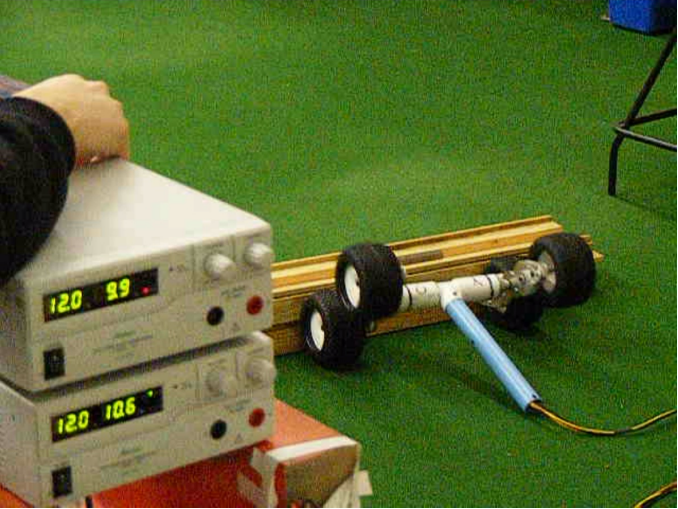
\includegraphics[width=0.35\textwidth]{Wilson-climbing}
	\caption{Wilson's half assembly climbing a stair \citep{Wilson-2013}.}
	\label{Wilson climbing}
\end{wrapfigure}

Wilson's robot had some limitations that prevented him from performing extensive tests. Chiefly, it was unable to climb stairs as the motors would stall upon encountering an obstacle. To validate the LIM concept in spite of this issue, Wilson split the robot in half and tested stair climbing using only the front LIMs and the chassis dragging behind as a tail. This "tail-dragging half assembly" was able to climb a single step as shown in Figure \ref{Wilson climbing}. Wilson's project ran out of time before he was able to solve the climbing motion of the complete robot, however he was able to confirm that the LIM system can climb at least a single stair in the half assembly configuration \citep{Wilson-2013}.

\subsection{Haskel's Theseus} %~~~~~~~~~~~~~~~~~~~~~~~~~~~~~~~~~~~~~~~~~~~~~~~~~~~~~~~~~~~~~~~~~

\begin{wrapfigure}{r}{0.35\textwidth}
	\centering
	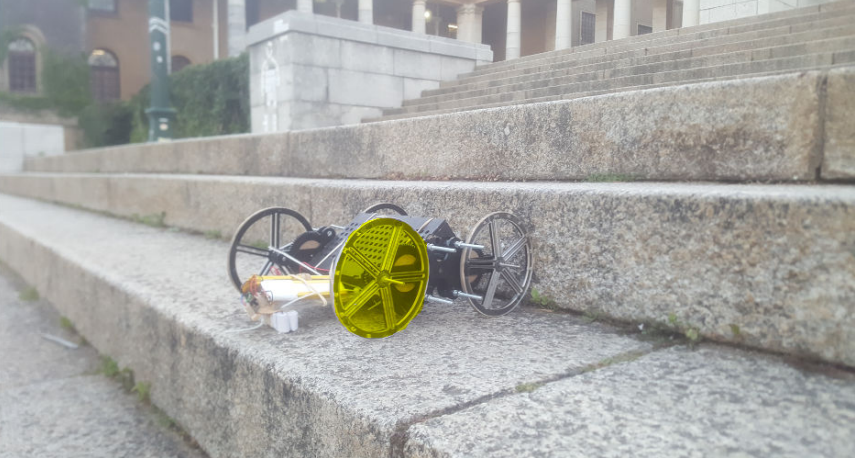
\includegraphics[width=0.35\textwidth]{Haskel-robot}
	\caption{Haskel's Theseus \citep{Haskel-2017}.}
	\label{Haskel robot}
\end{wrapfigure}
Haskel designed and built a LIMed robot to further test the concept, which he named "Theseus", shown in Figure \ref{Haskel robot}. Unlike Wilson, Haskel assumes that using LIMs for rear wheels is not necessary for the stair climbing motion, and instead chooses to use a dragging tail to provide counter torque, similar to the tail-dragging half assembly used by Wilson. Theseus is much smaller and lighter than Wilson's robot.\\

Haskel tested different concepts for the tire tread, dragging tail, and gear ratios. However, none of his configurations could consistently climb a step. In the majority of step-climbing attempts, Theseus' LIMs would flip over to mount the step, but it would not be able to pull itself up. This can be attributed to a lack of grip or a lack of torque. Haskel intended to do further work on the project, however he ran out of time due to component shortages and protests at UCT \citep{Haskel-2017}.
\newpage
\subsection{Buchanan's Ascender} %~~~~~~~~~~~~~~~~~~~~~~~~~~~~~~~~~~~~~~~~~~~~~~~~~~~~~~~~~~~~~~~~~

\begin{wrapfigure}{r}{0.35\textwidth}
	\centering
	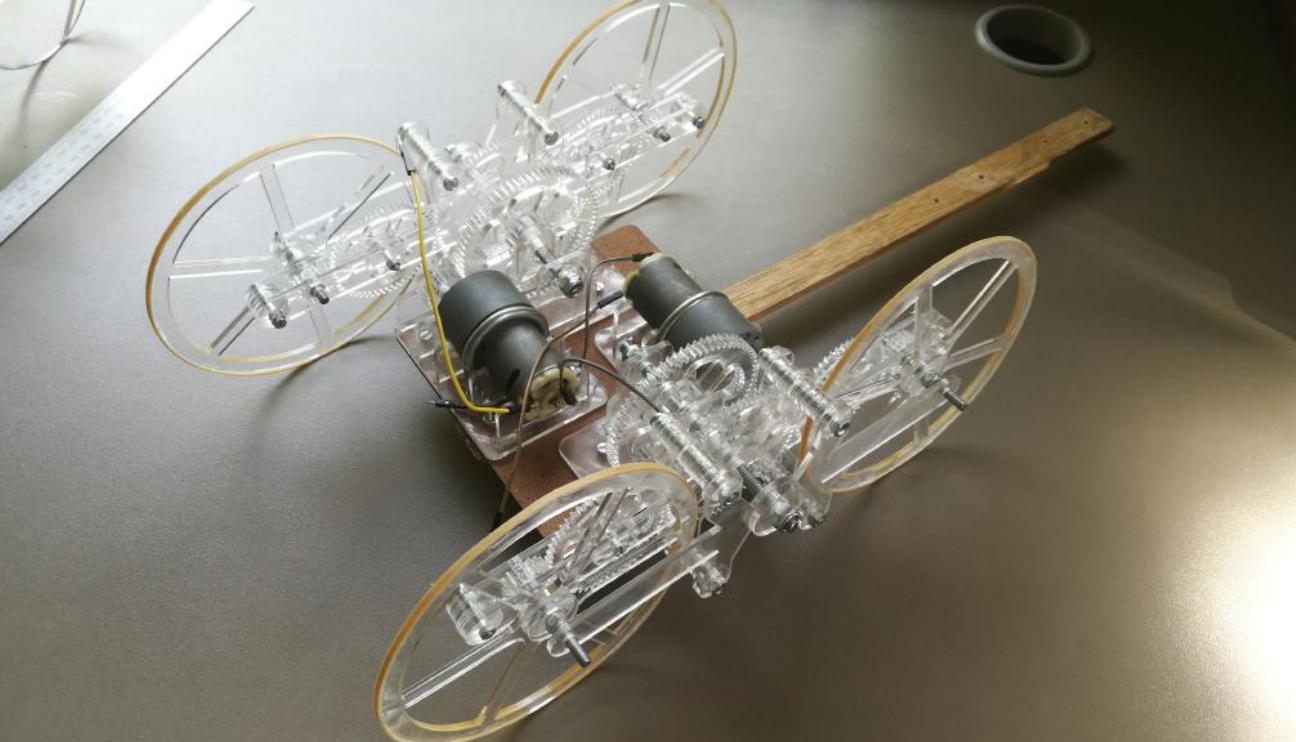
\includegraphics[width=0.35\textwidth]{Buch-robot}
	\caption{Buchanan's Ascender \citep{Buchanan-2018}.}
	\label{Buch robot}
\end{wrapfigure}
Buchanan designed and built "Ascender", a robot platform using LIMs for locomotion, shown in Figure \ref{Buch robot}. Buchanan iterated on the design several times in order to reduce mass and increase torque. The intention was to build a drivetrain that could be combined with the electronics of Haskel's Theseus to produce a successful stair climbing robot. As such, the Ascender does not include any electronic control systems, and is instead controlled externally by power supplies connected to the motors.

Buchanan's testing showed that the Ascender was able to climb a single step of 120 mm in 6 out of 10 attempts, and a step of 140mm in 2 out of 10 attempts. Buchanan noted a flaw in the design; after the LIMs flip over as part of the climbing motion, the body of the robot would lodge itself onto the edge of the step and the wheels would spin freely, a phenomenon referred to as beaching. The LIMs would then spin until the top wheel makes contact with the top of the step, from there it would either grip and pull the robot up the step as intended, or it would dislodge the body and the robot would fall off the step. Buchanan also reported that the Ascender was fragile to the point that it broke during the testing. Buchanan did not test the Ascender's ability to climb a staircase, but he concluded that it would be able to as a staircase is simply repeated single steps. \citep{Buchanan-2018}

\subsection{Powrie's Di-Wheel robot}

\begin{wrapfigure}{r}{0.35\textwidth}
	\centering
	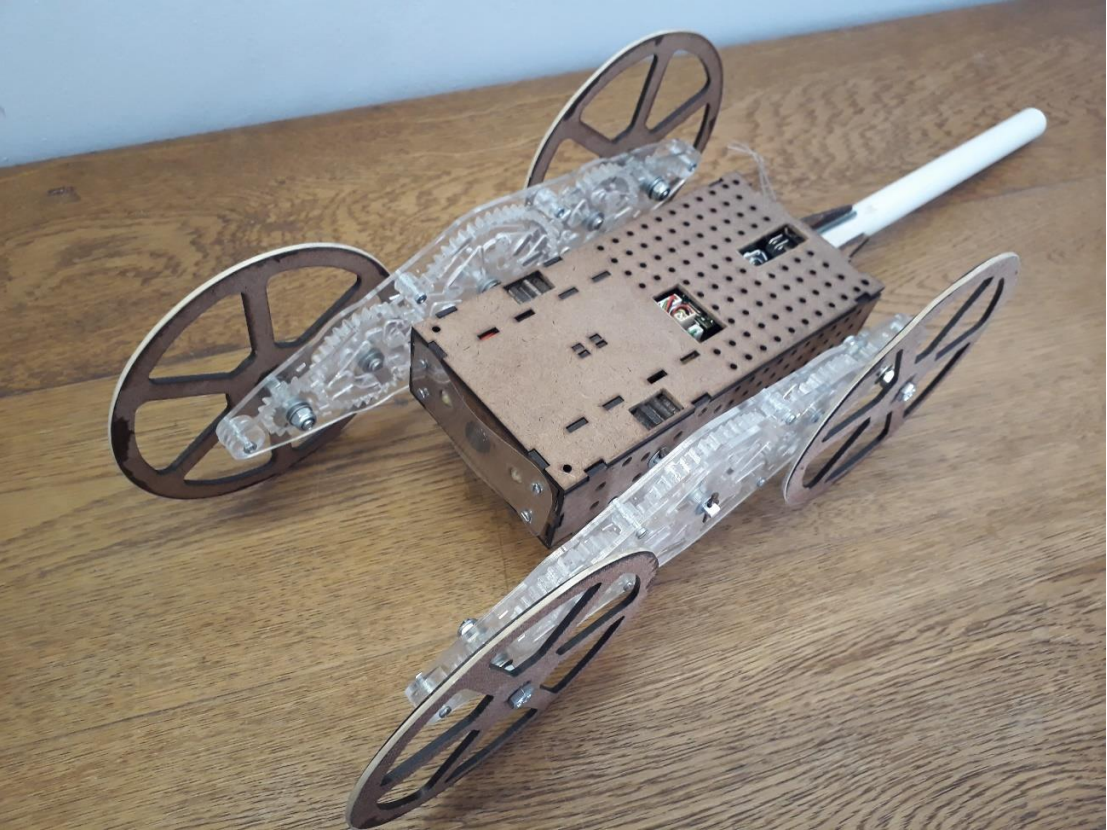
\includegraphics[width=0.35\textwidth]{Powrie-device}
	\caption{Powrie's Di-Wheel Robot \citep{Powrie-2019}.}
	\label{fig:Powrie robot}
\end{wrapfigure}
Powrie developed a robot using LIMs, however in his report he referred to LIMs as Di-Wheels. His reason for renaming them is that the behaviour of the LIMs does not only respond to external loads on the wheels, it also depends on the torque applied by the motors. He chose the name "Di-Wheel" in reference to a similar design by the name of "Tri-Wheel", which used three minor wheels instead of two, developed by \cite{Smith-2015}. Powrie's Di-Wheel robot is larger and more robust than Buchanan's Ascender, while being lighter than Wilson's LIMed robot. It is shown in Figure \ref{fig:Powrie robot}.\\


The Di-Wheel robot was successful in climbing a single step of 220 mm. Further testing was not performed as noise from the robot's motors would interfere with the control system, preventing untethered driving. Powrie ran out of time before he was able to solve this issue. Powrie also found that when both motors are powered on, one of the LIMs would flip first, putting all the weight on the other LIM so preventing it from flipping. The result is that the robot would fall on its side, as seen in Figure \ref{Powrie falling} \citep{Powrie-2019}.\\
\begin{figure}[ht]
	\centering
	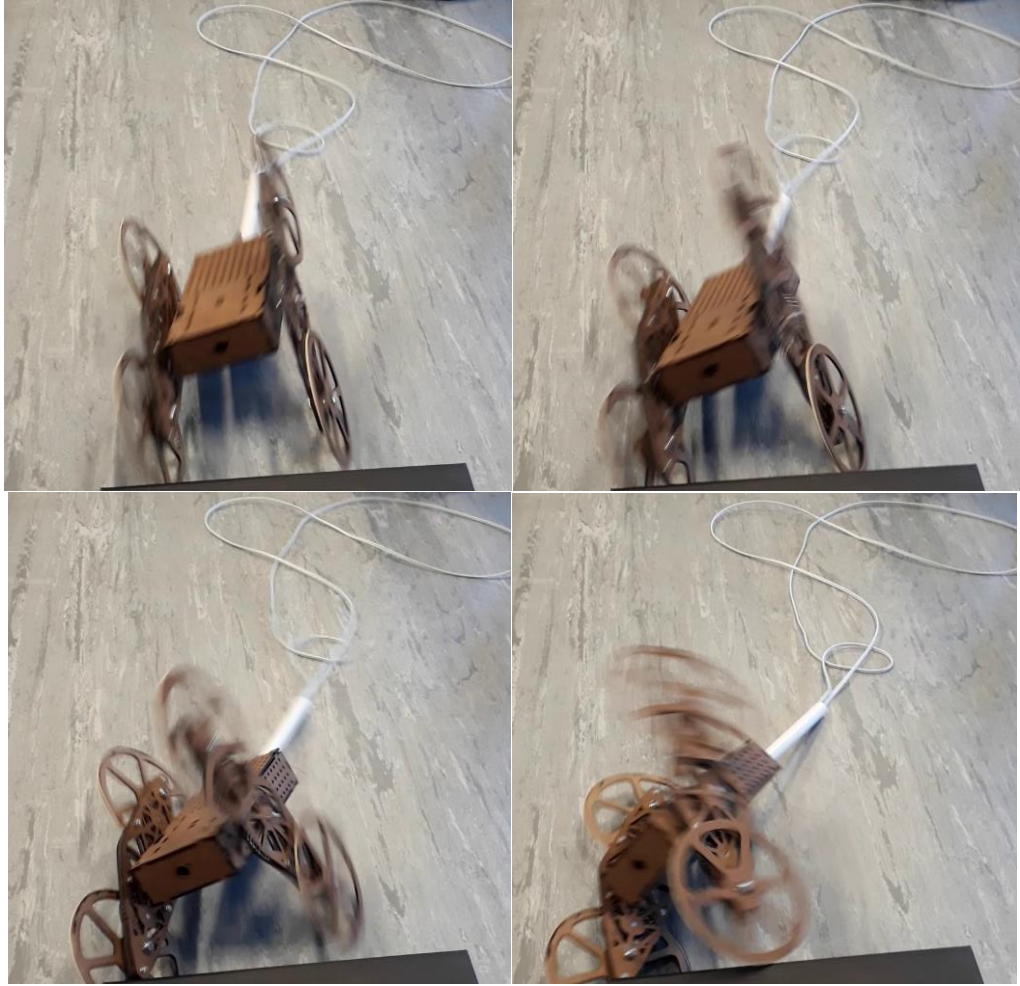
\includegraphics[width=0.5\textwidth]{Powrie-falling}
	\caption{The Di-Wheel robot falling due to unsynchronised LIMs \citep{Powrie-2019}.}
	\label{Powrie falling}
\end{figure}


\subsection{Gearing} %~~~~~~~~~~~~~~~~~~~~~~~~~~~~~~~~~~~~~~~~~~~~~~~~~~~~~~~~~~~~~~~~~
%Add drawing!!
The gear ratios of the LIMs will affect its motion significantly. The rotational speed of the central gear will be translated into both the speed of the LIM frame and the speed of the wheels:
\begin{align*}
	\dot{\theta}_{\mathrm{Sun}} &= \dot{\theta}_{\mathrm{Frame}} + \frac{N_\mathrm{Planet}}{N_\mathrm{Sun}}\dot{\theta}_{\mathrm{Planet}} \tag{1}\\
\end{align*}
where $\dot{\theta}_{\mathrm{Sun}}$ is the angular speed of the central gear, $\dot{\theta}_{\mathrm{Frame}}$ is the angular speed of the LIM frame, $\dot{\theta}_{\mathrm{Planet}}$ is the angular speed of the outer gears and wheels relative to the frame, $N_{\mathrm{Planet}}$ is the number of teeth on the outer gears, and $N_\mathrm{Sun}$ is the number of teeth on the central gear.\\

When both the wheels and the LIM frame aren't constrained, the system is under-actuated and its motion is non-trivial. In the case that the LIM frame isn't flipping (i.e. normal driving on a flat plane), $\dot{\theta}_{\mathrm{Frame}} = 0$, therefore:\\
 \begin{align*}
 	\dot{\theta}_{\mathrm{Planet}} &= \frac{N_\mathrm{Sun}}{N_\mathrm{Planet}}\dot{\theta}_{\mathrm{Sun}} \tag{2}\\
 \end{align*}
When the wheels have encountered an obstacle, such as a step, friction will prevent them from turning, $\dot{\theta}_{\mathrm{Planet}} + \dot{\theta}_{\mathrm{Frame}} = 0$. In this case:
\begin{align*}
	\dot{\theta}_{\mathrm{Frame}} &= \frac{\dot{\theta}_{\mathrm{Sun}}}{(1-\frac{N_\mathrm{Planet}}{N_\mathrm{Sun}})} \tag{3}\\
\end{align*}

This means that during flipping motion, if $\frac{N_\mathrm{Planet}}{N_\mathrm{Sun}} > 1$, then the LIM frame will flip in the opposite direction to the rotation of the central gear, so the front wheel will roll up the side of the obstacle \citep{Wilson-2013}. This is ineffective for climbing steps as the LIM will never mount the step, but rather continue rotating backwards until it returns to the starting position \citep{Haskel-2017}.\\

\begin{figure}[h]
	\centering
	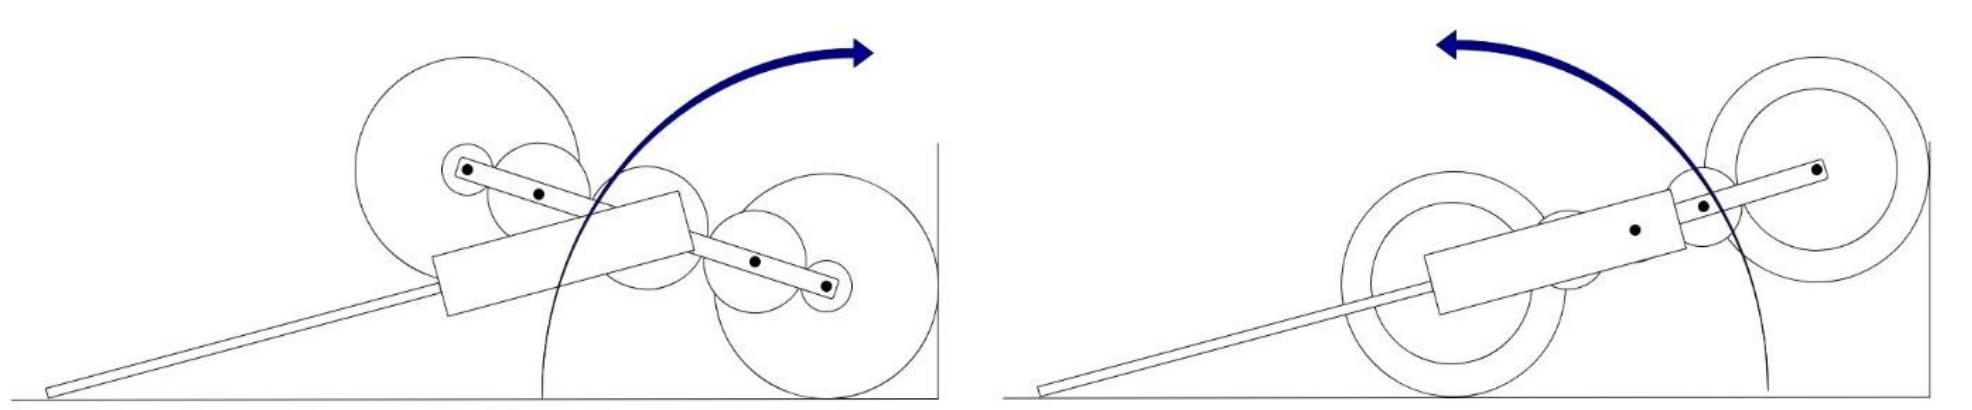
\includegraphics[width=0.9\textwidth]{Powrie-gear-differences}
	\caption{Two different climbing motions using different gear ratios \citep{Powrie-2019}.}
	\label{Powrie gears}
\end{figure}

If $\frac{N_\mathrm{Planet}}{N_\mathrm{Sun}} < 1$, then the LIM frame will rotate forward, the rear wheel will flip over and mount the obstacle. This allows the LIM to climb stairs as intended.\\
The two cases are shown in Figure \ref{Powrie gears}, with the left showing the case when $\frac{N_\mathrm{Planet}}{N_\mathrm{Sun}} < 1$, and the right showing the case when $\frac{N_\mathrm{Planet}}{N_\mathrm{Sun}} > 1$.



%\subsection{Control requirements} %~~~~~~~~~~~~~~~~~~~~~~~~~~~~~~~~~~~~~~~~~~~~~~~~~~~~~~~~~~~~~~~~~
%
%LIMs are considered "Load intuitive" because of their ability to adapt to terrain mechanically. Open-loop control is ideal in this case, as an operator need only turn the motor on and the LIM will drive forward if it can, or attempt to climb an obstacle if it is obstructed \citep{Wilson-2013}. However, Powrie found that his robot was not suited to open loop control. When full voltage is provided to the motor, the LIMs would flip even if when is on a flat plane. Powrie's calculations suggest that whether the LIM flips or not is largely dependent on the torque applied to it. A low torque results rolling, and a high torque results in flipping. His report suggests that LIMs only responds to terrain intuitively for a "medium torque" \citep{Powrie-2019}. In this case a medium torque would be defined as a torque that results in rolling when the LIM is unobstructed, and flipping only when it is obstructed. This indicates that it may be necessary to have a control system that manages the torque provided to the LIMs to ensure that they do not flip on flat terrain if the motors are sufficiently powerful.\\
%
%Powrie also found that when climbing a step, one LIM could flip first, putting weight on the other and preventing it from flipping, as seen previously in Figure \ref{Powrie falling} \citep{Powrie-2019}. This suggest that a control system is needed to roughly synchronise the LIMs, if one is ahead of the other, more torque should be provided to the trailing LIM to correct its motion.
\chapter{2D simulation}

In order to create an accurate model of the LIM system, it is important to understand how it functions. Previous reports have given some insight into this, but none of them have demonstrated a LIM robot that can climb consecutive steps. Wilson performed a simple simulation of a LIM robot in Algodoo, and concluded that the robot would need LIMs for the rear wheels in order to support consecutive stair climbing \citep{Wilson-2013}, however all of the subsequent projects simply used a dragging tail instead of rear wheels. There is a need to resolve this inconsistency in past work, and to gain insight into the function of the LIM system. To do this, another 2D simulation using Algodoo is performed.

\section{Limitations}

Algodoo is a two dimensional physics sandbox \citep{Algodoo}. Initial testing with the software showed that limitations on the physics engine prevent accurate simulation of gears with teeth at a centimetre scale. This means it is impossible to accurately simulate a LIM device at the scale that they would be used in reality. The simulation can be scaled up to avoid this issue. However, this prevents an accurate simulation of the kinematics of the system.\\

Additionally, it was found that Algodoo does not allow for the accurate simulation of an electric motor. In a typical electric motor, the available torque will decrease as the speed increases. This nuance is not present in Algodoo, so it cannot be used to provide an accurate simulation of the motor requirements. Despite these limitations. Algodoo is still useful as a tool to roughly test the motion of LIMs, and to determine how it would interact with steps. The advantage of Algodoo over other simulation methods is its ease of use, it only takes a few minutes to build a LIMed robot in Algodoo.

\section{Configuration}


To improve the accuracy of the Algodoo physics engine, the simulation frequency is set to 1200 and all objects are scaled up 100 times. A basic LIM system with a dragging tail is set up, using gear and wheel dimensions from \cite{Powrie-2019}, shown in Figure \ref{algo-model}.

\begin{figure}[h]
	\centering
	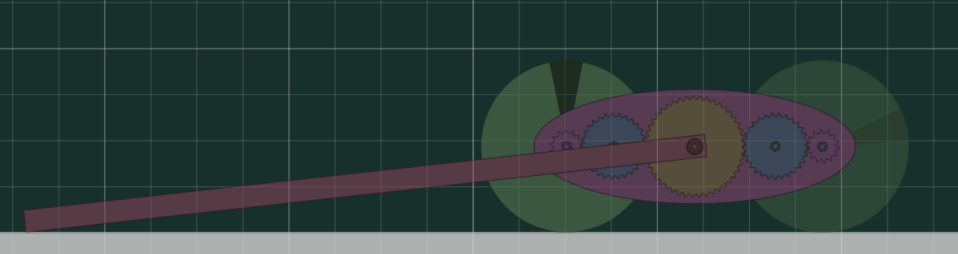
\includegraphics[width=0.8\textwidth]{algo-model}
	\caption{Initial Algodoo LIM system}
	\label{algo-model}
\end{figure}
\section{Observations}

\subsection{Rear wheels}

Simulations suggest that rear wheels are not necessary for successful consecutive stair climbing. If the motor torque is sufficient, the LIM will be able to climb steps with only a dragging tail for counter torque. It should be noted that adding a motorised rear wheel, with or without LIMs, does provide a supporting force to the front LIMs during flipping motion, so if the frontal motor cannot provide sufficient torque, rear wheels should be considered in the design.

\subsection{Mounting obstacles}

There are three ways in which a LIM can mount an obstacle after flipping up to it. The first is that the wheel collides directly with the obstacle, shown in Figure \ref{algo-case-wheel}. This happens when the obstacle is taller than a certain threshold based on the geometry of the LIM, and can result in the wheel bouncing off of the obstacle and failing to pull itself up. In this case a controller may be used to limit the speed of the flipping motion to ensure that the wheel is not going fast enough to bounce off the obstacle when it collides. \\

\begin{figure}[h]
	\centering
	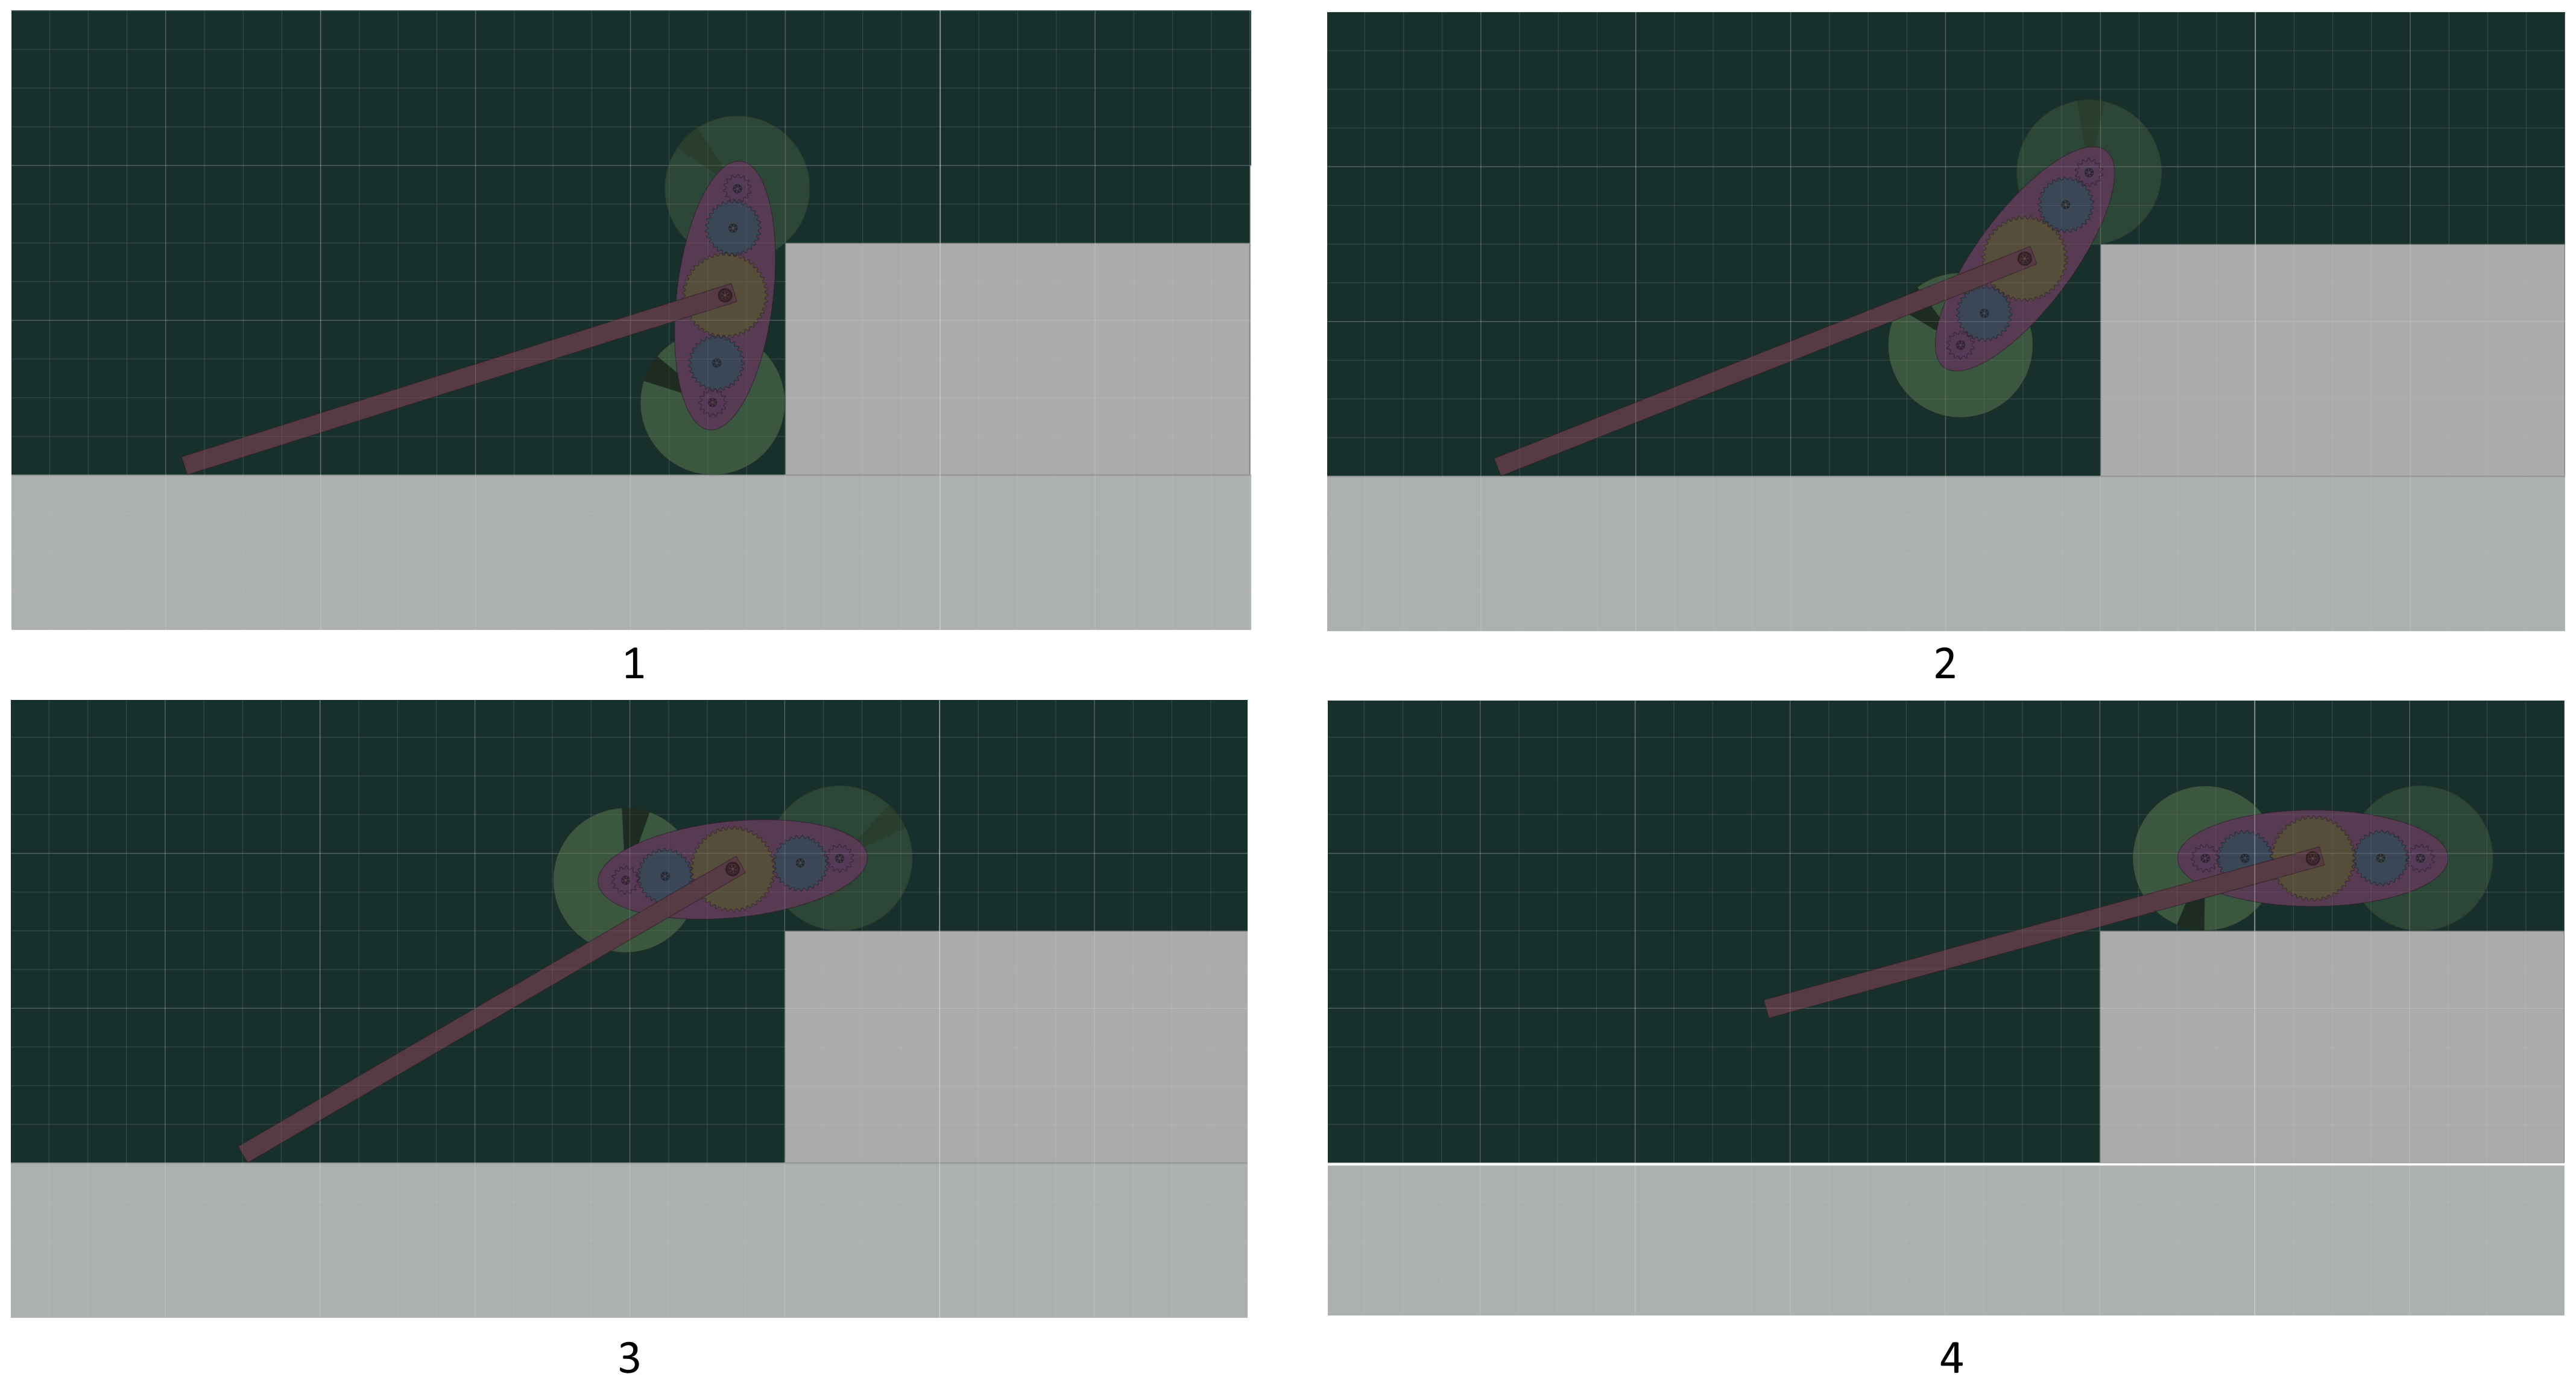
\includegraphics[width=0.8\textwidth]{algo-case-wheel}
	\caption{LIM climbing with wheel contact}
	\label{algo-case-wheel}
\end{figure}

The second way is that the LIM frame collides with the obstacle and mounts it, then the LIM continues to rotate until the wheel makes contact with the surface of the obstacle to pull the robot forward. This case is shown in Figure \ref{algo-case-frame}. Note that the LIM frame can slip on the edge of the obstacle, which may result in failure to climb. \\

\begin{figure}[h]
	\centering
	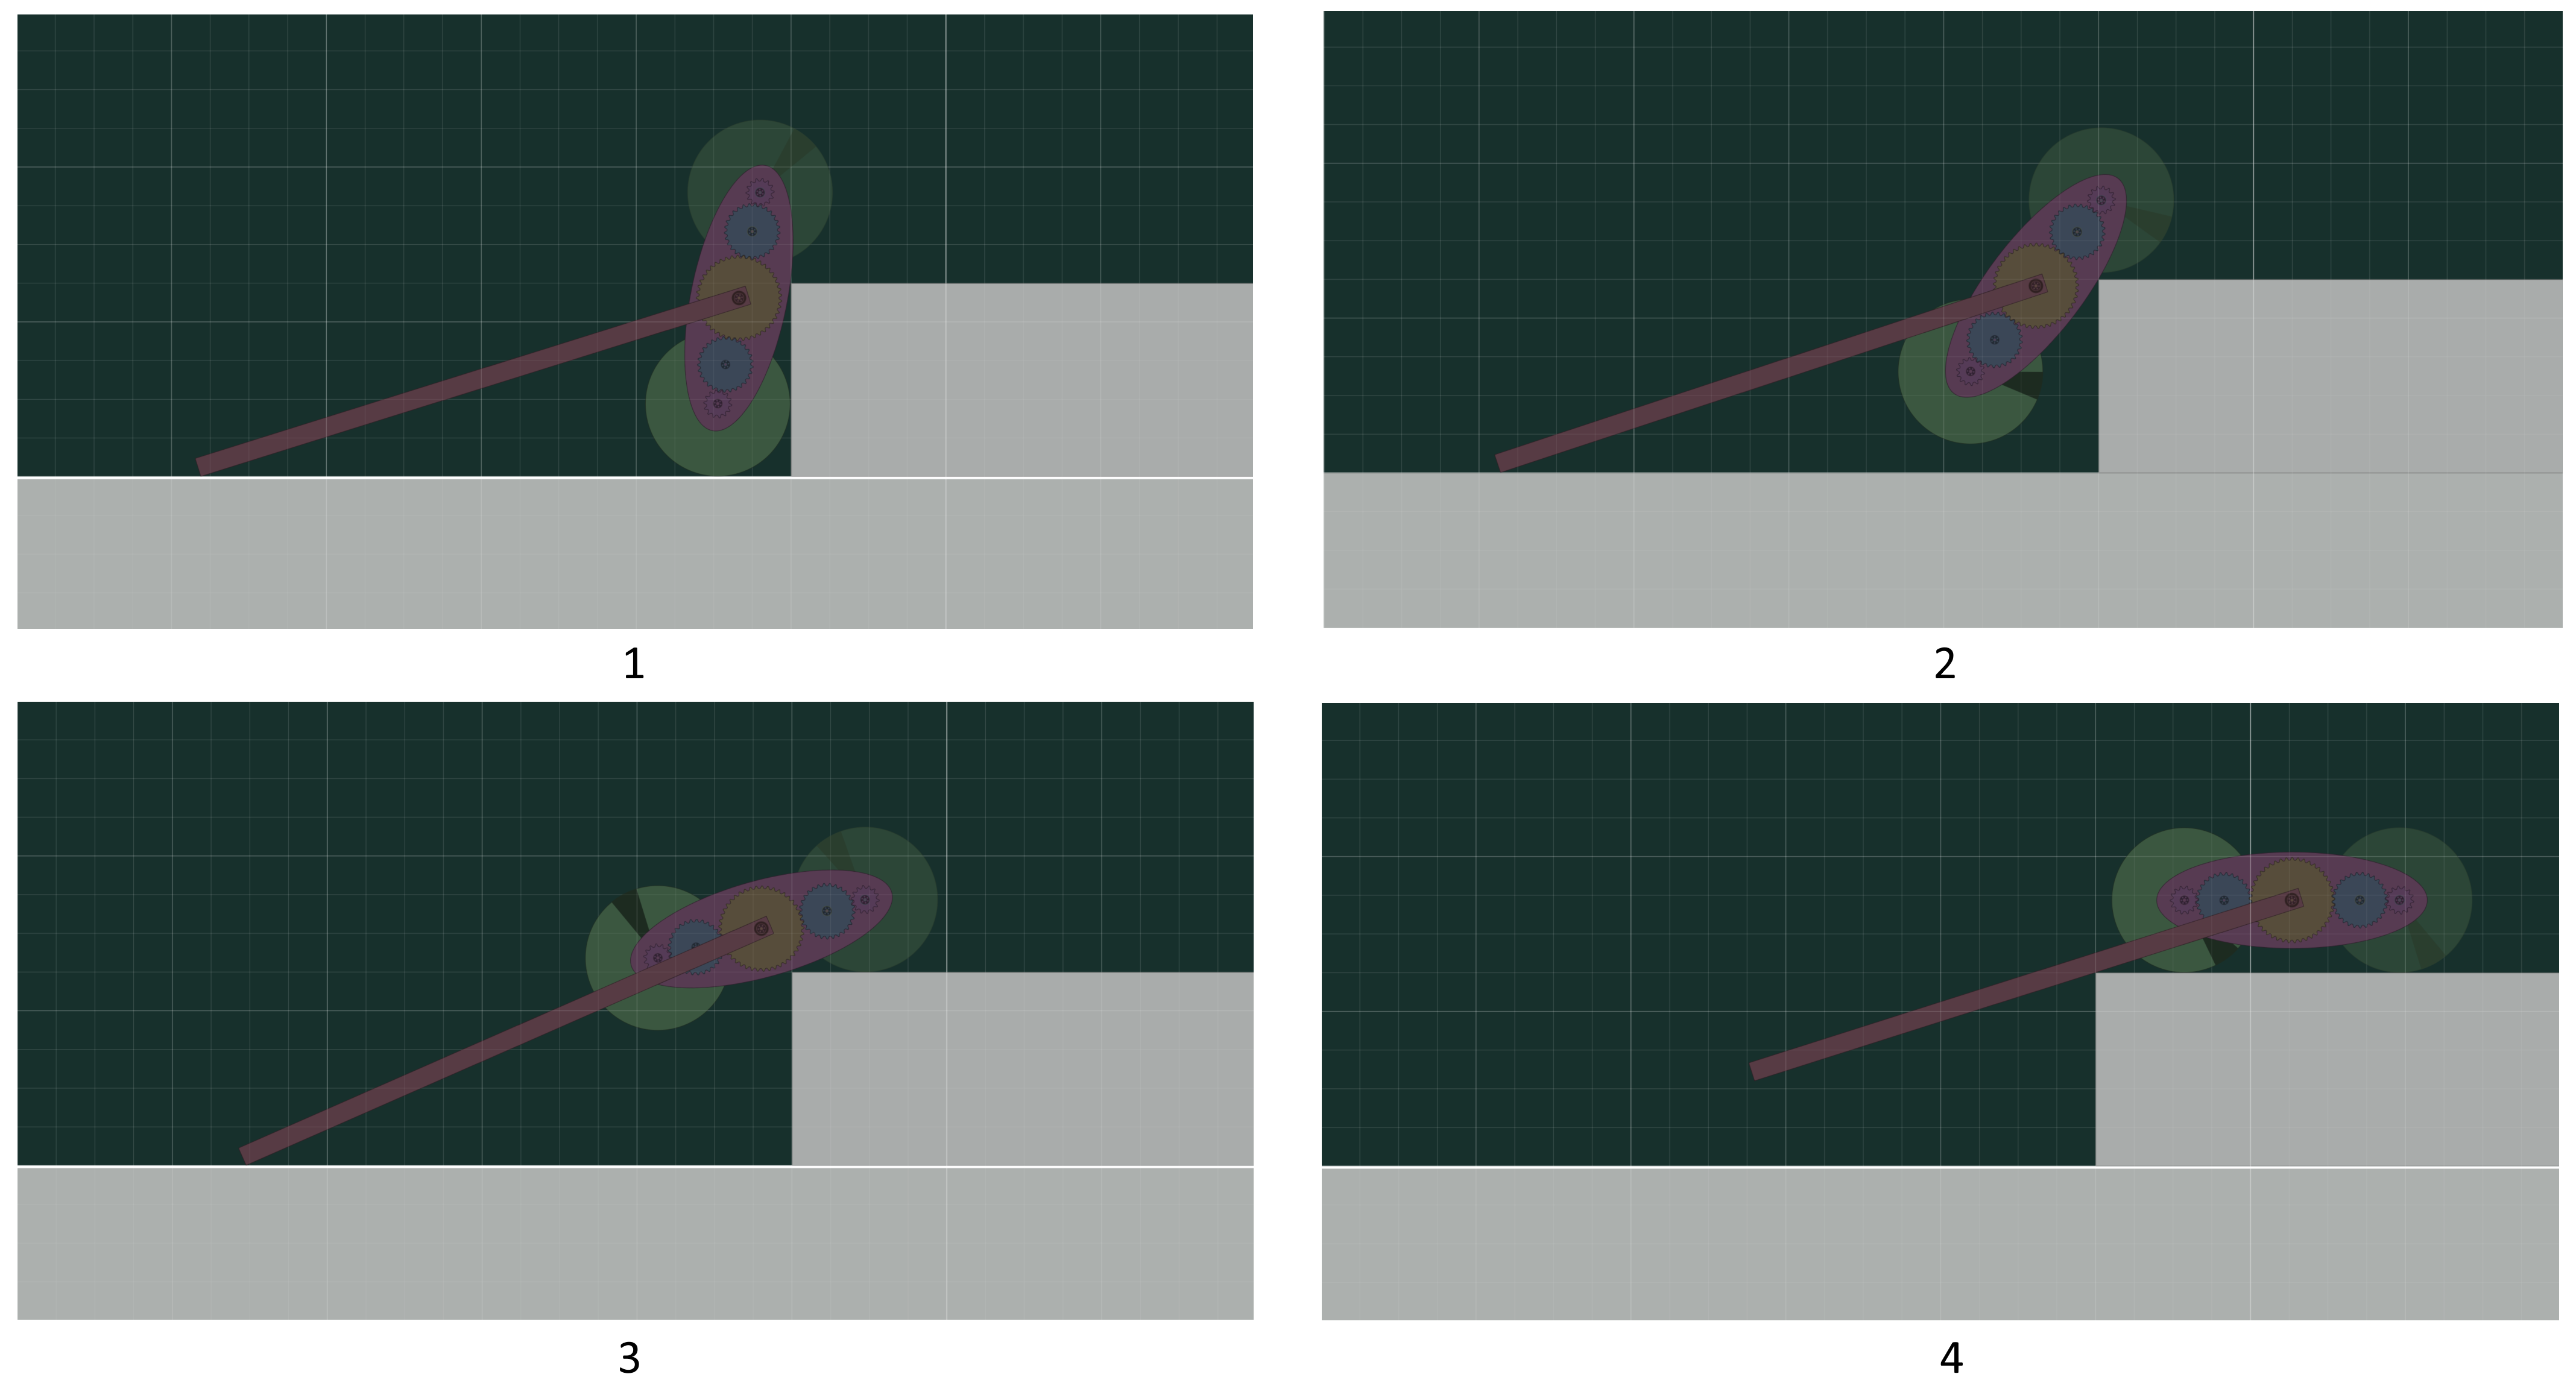
\includegraphics[width=0.8\textwidth]{algo-case-frame}
	\caption{LIM climbing with LIM frame contact, note how the contact point slips between 1 and 2}
	\label{algo-case-frame}
\end{figure}

The third way is that the body of the robot, presented here as an extension of the tail, will mount the obstacle. This is shown in Figure \ref{algo-case-body}. When the body has beached onto the obstacle, seen in Figure \ref{algo-case-body}.2, there is nothing resisting the motion of either the wheels or the LIM, so they can accelerate quite quickly. If they move too fast, the wheel can bounce off the obstacle when it makes contact, dislodging the body so that it falls back down to the initial position. \cite{Buchanan-2018} found that his Ascender followed this motion, which caused it to fail many of its climbing tests. He mentions that this can be avoided by moving the LIM axle to the end of the body, so that the body does not protrude beyond the LIM frame during climbing motion.\\

\begin{figure}[h]
	\centering
	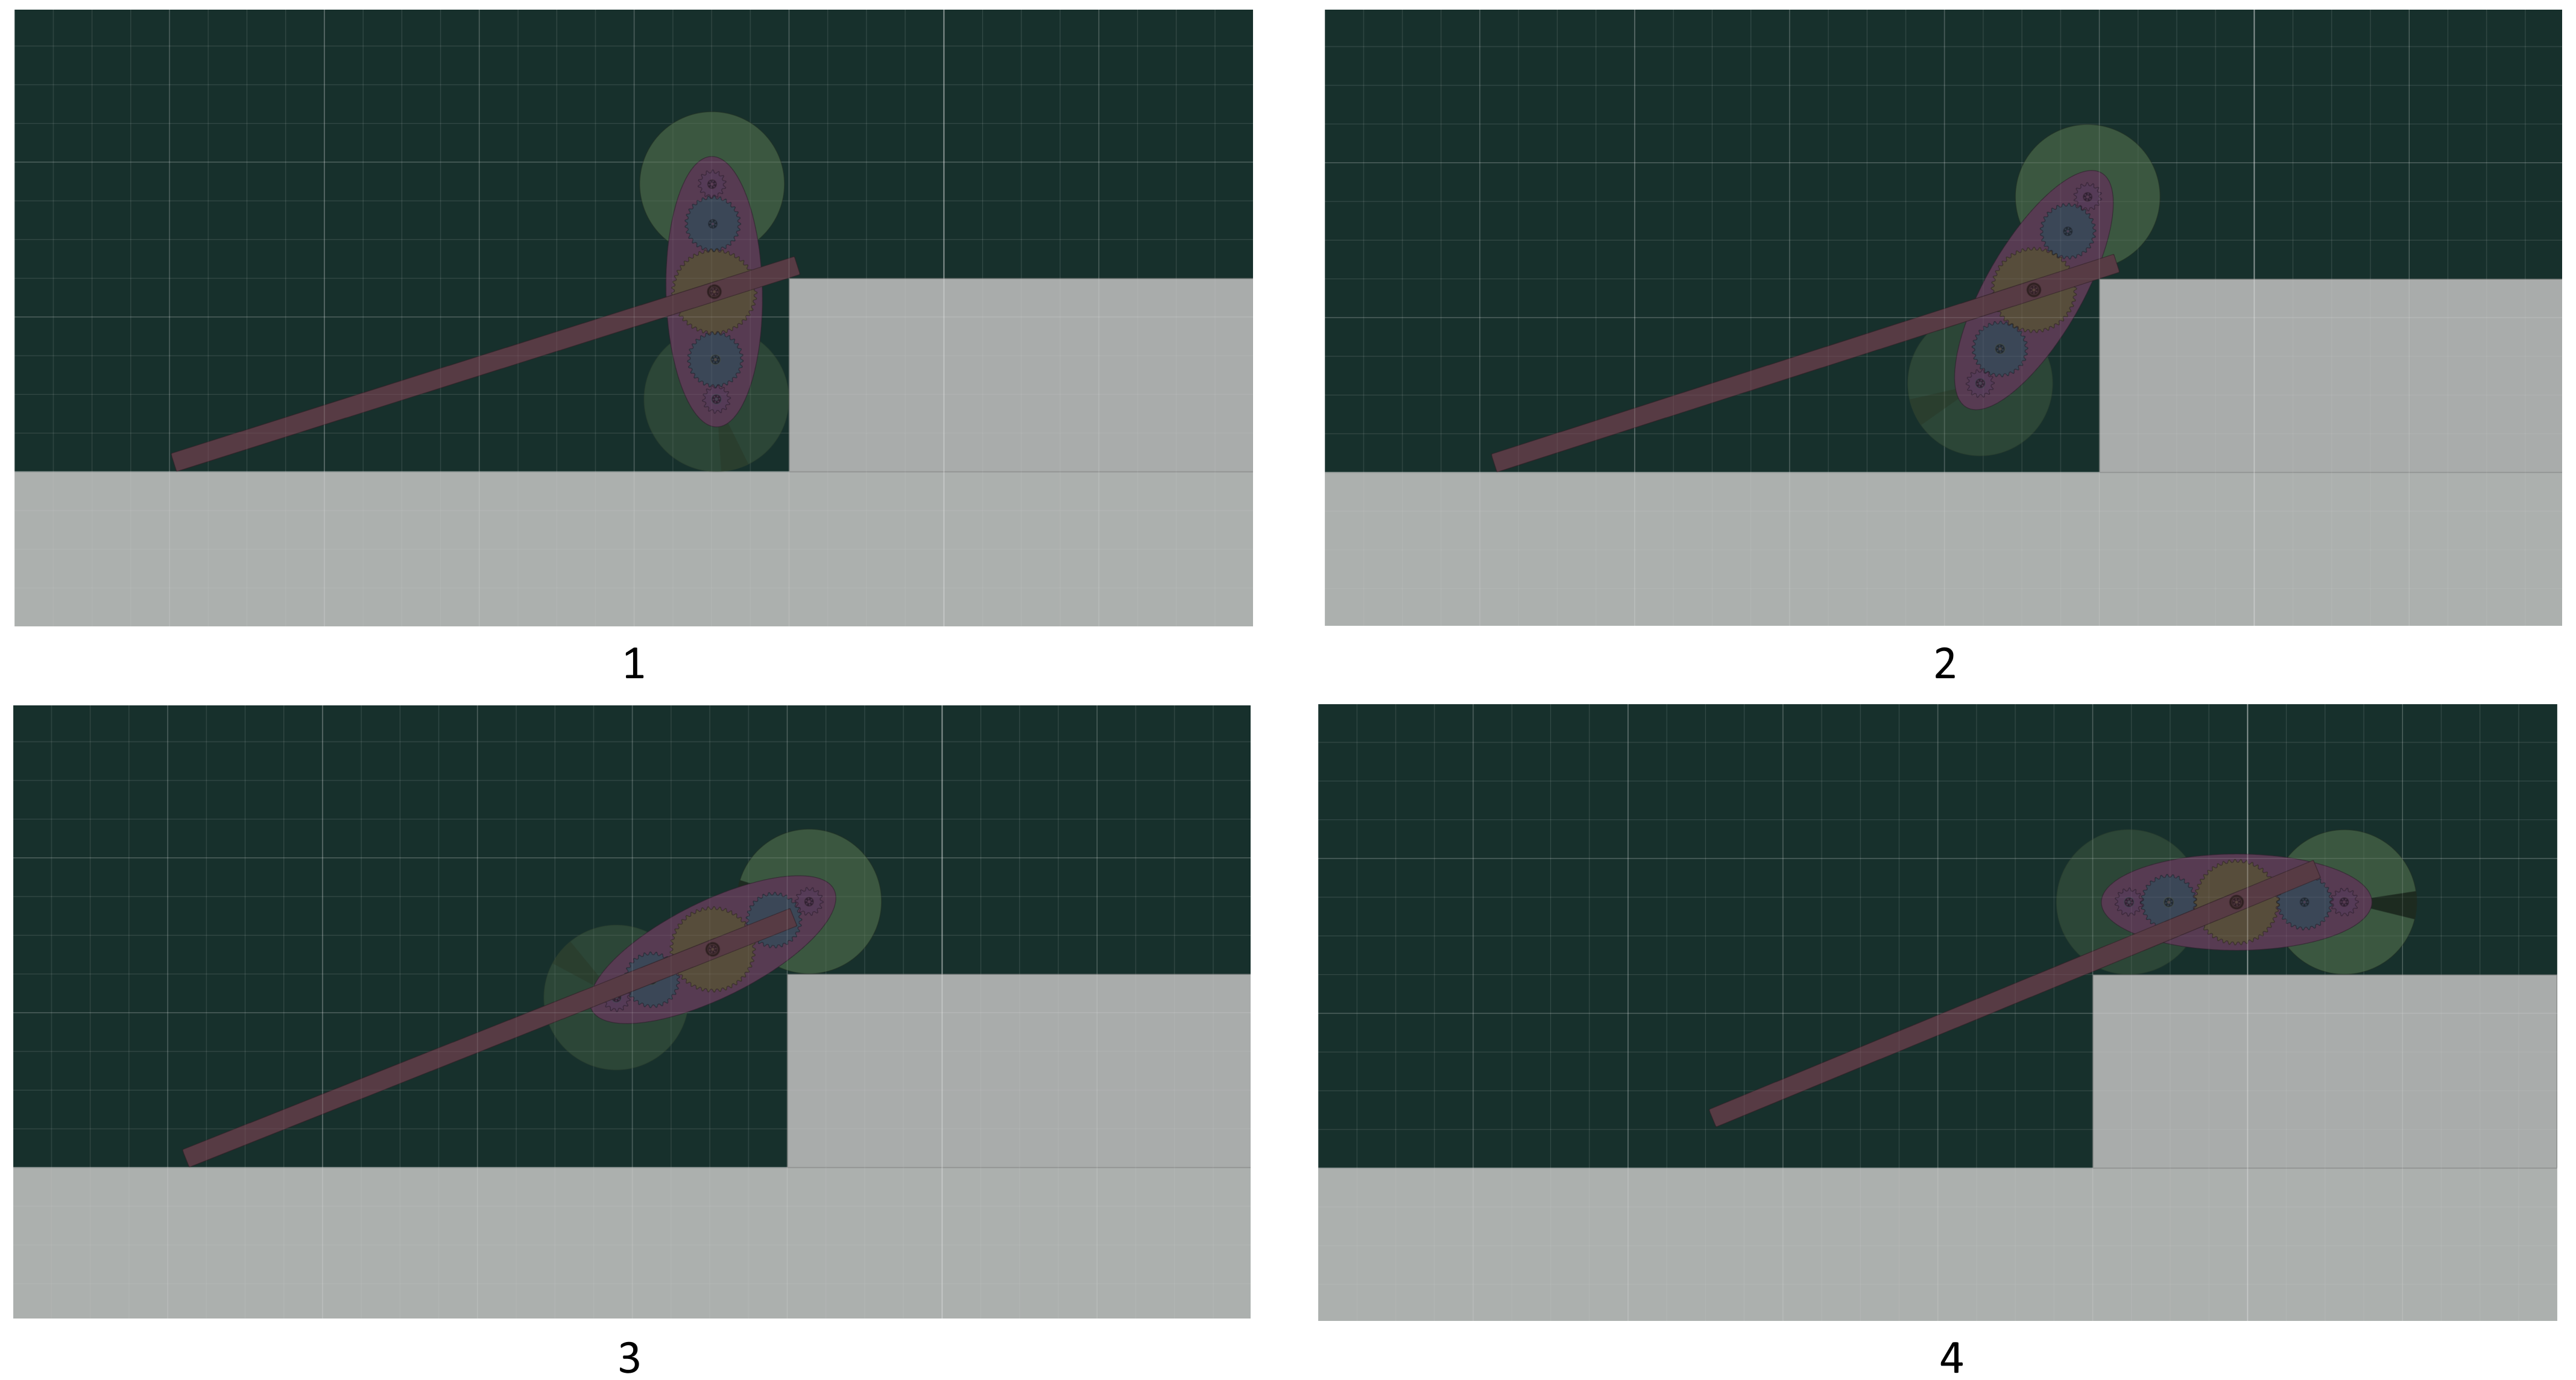
\includegraphics[width=0.8\textwidth]{algo-case-body}
	\caption{LIM climbing with robot body contact}
	\label{algo-case-body}
\end{figure}

Each of these climbing methods has its flaws, however the case where the LIM frame collides with the obstacle is preferred as it reduces the chance that the wheel will bounce off the obstacle. To address slipping, grousers can be added to the robot's body \citep{rob2014}. The updated model with grousers can be seen in Figure \ref{algo-model2}.\\

\begin{figure}[h]
	\centering
	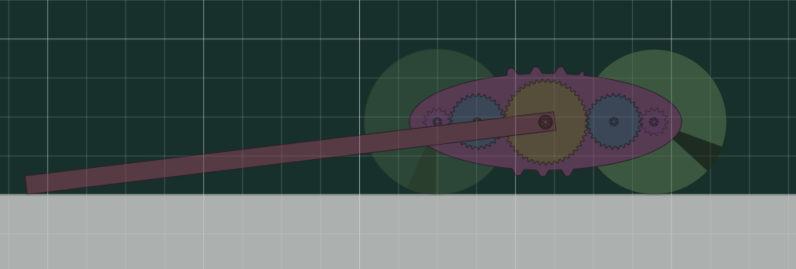
\includegraphics[width=0.8\textwidth]{algo-model2}
	\caption{Algodoo LIM system with grousers on frame}
	\label{algo-model2}
\end{figure}

\subsection{Rolling and flipping}

It was observed in simulation that the LIM would either roll or flip depending on the torque applied to it. There appeared to be a very small range of "medium torque" at which the LIM was truly load intuitive, if the motor torque was too weak it would never be able to flip over the obstacle and if it was too strong it would always flip and never roll, which hinders movement on flat terrain. However, this may simply be a result of inaccuracies of the simulation, as scaling and poor motor physics could significantly affect this motion. \\

In reality, as an electric motor increases in speed, the torque available will decrease proportionally. This means that once the LIM is rolling at speed, it will no longer have enough torque to flip itself unless it is stopped by an obstacle. This suggests that too much torque will only cause unintended flipping when the LIM is at rest on a flat plane.\\

\begin{figure}[h]
	\centering
	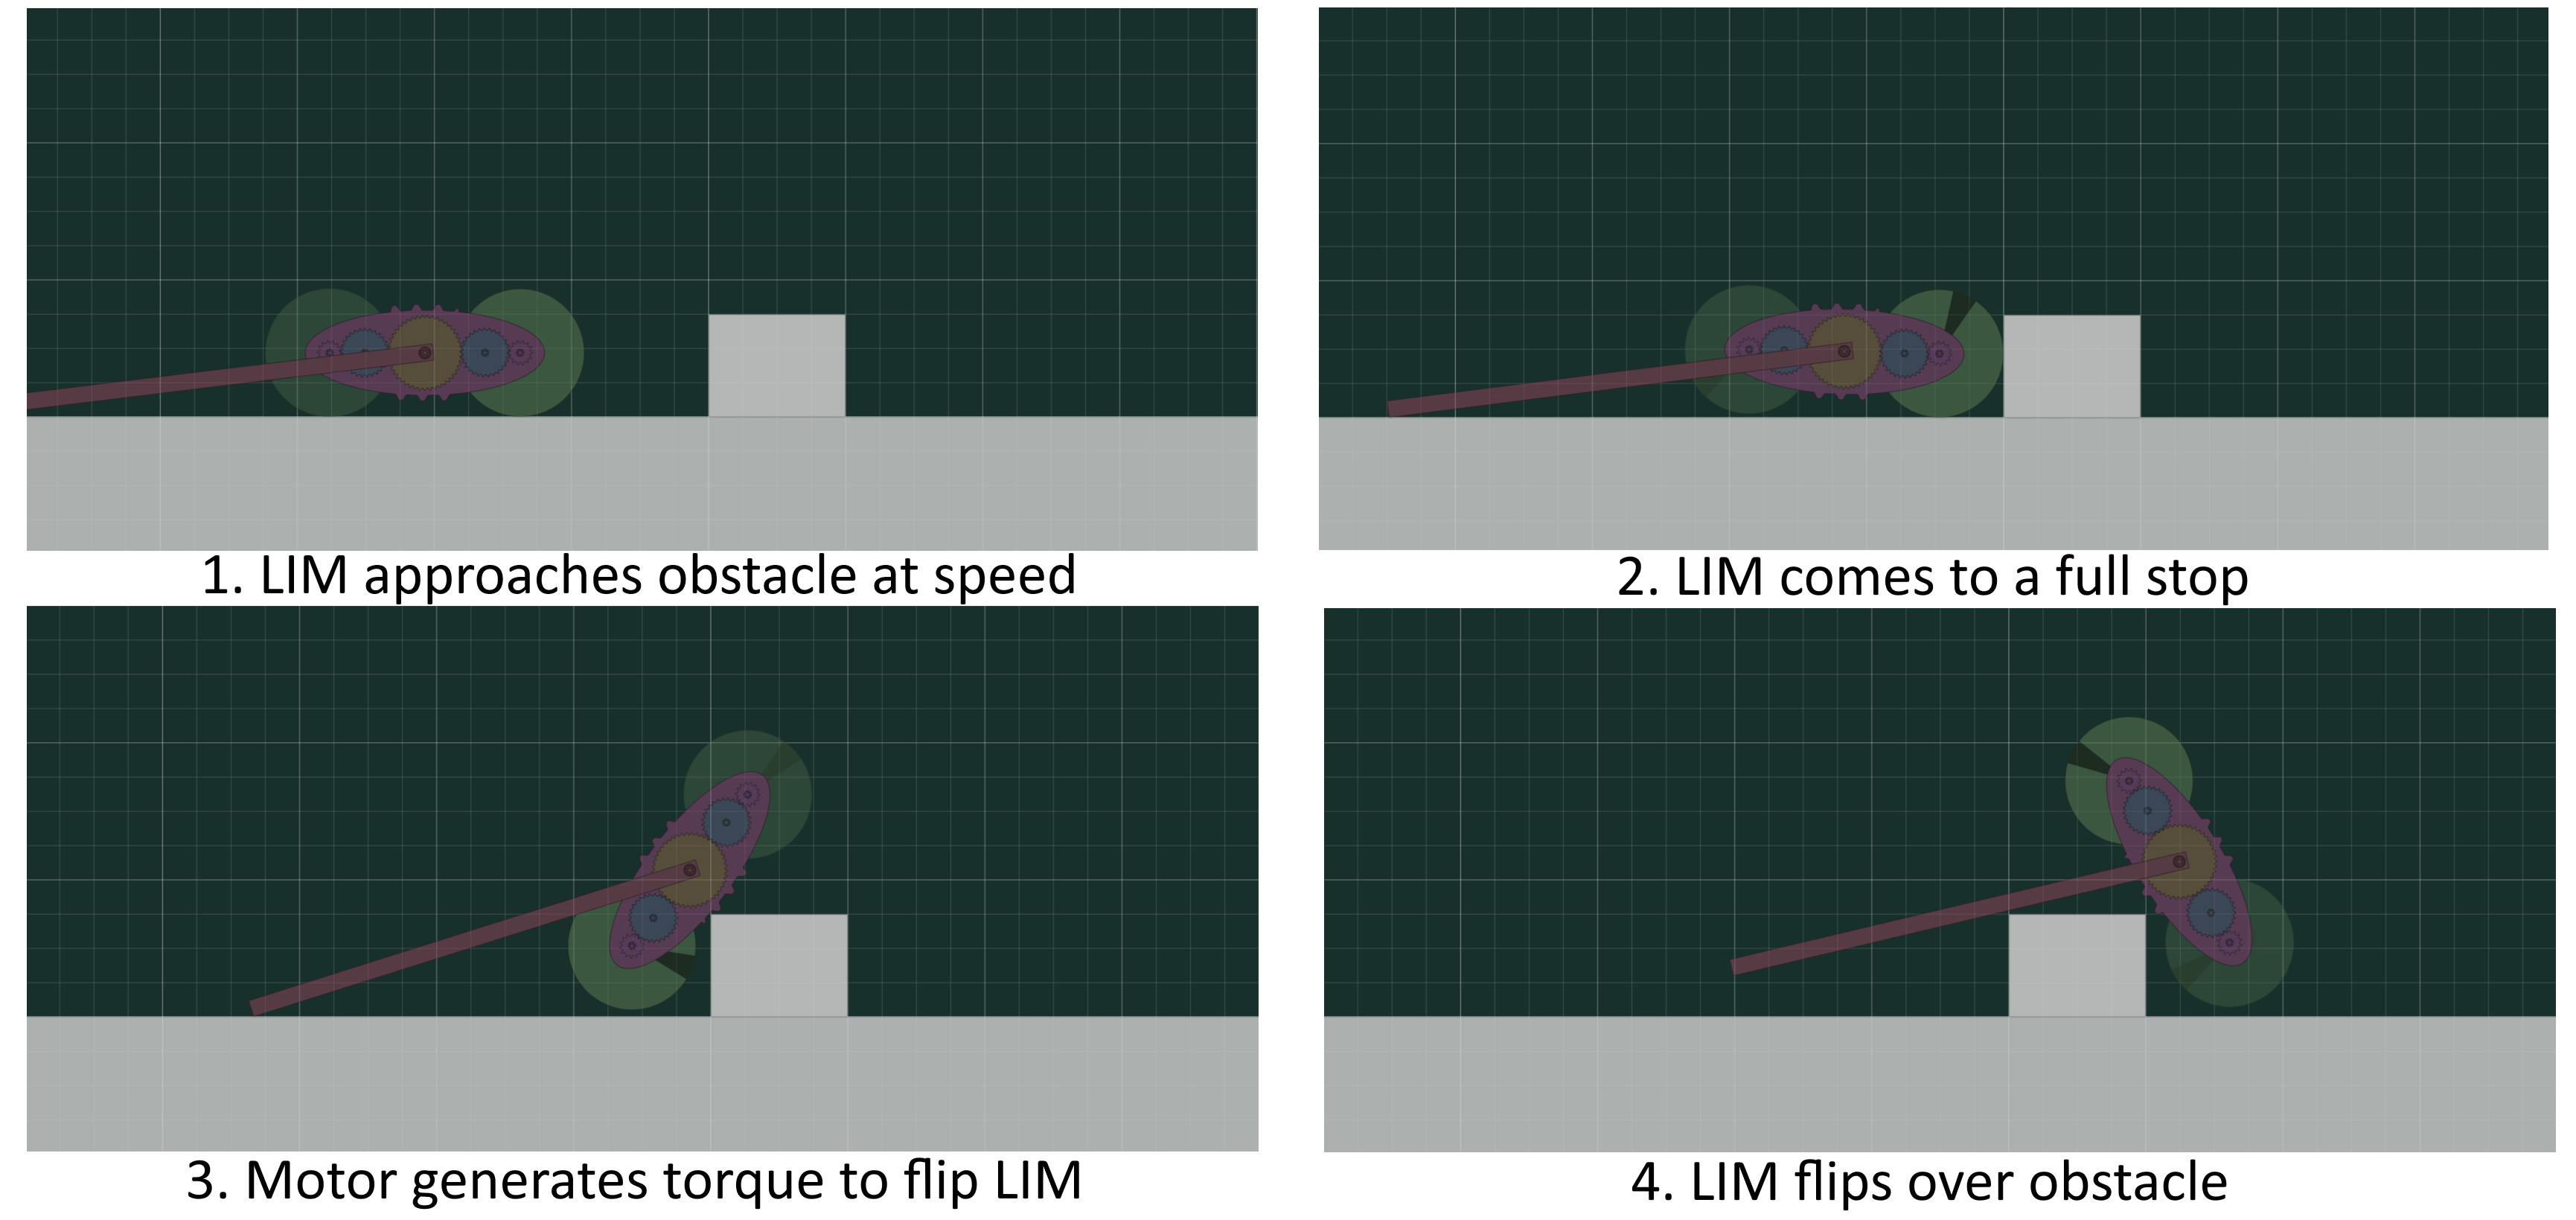
\includegraphics[width=1\textwidth]{algo-hori}
	\caption{Algodoo LIM system approaching obstacle horizontally}
	\label{algo-hori}
\end{figure}

\begin{figure}[h]
	\centering
	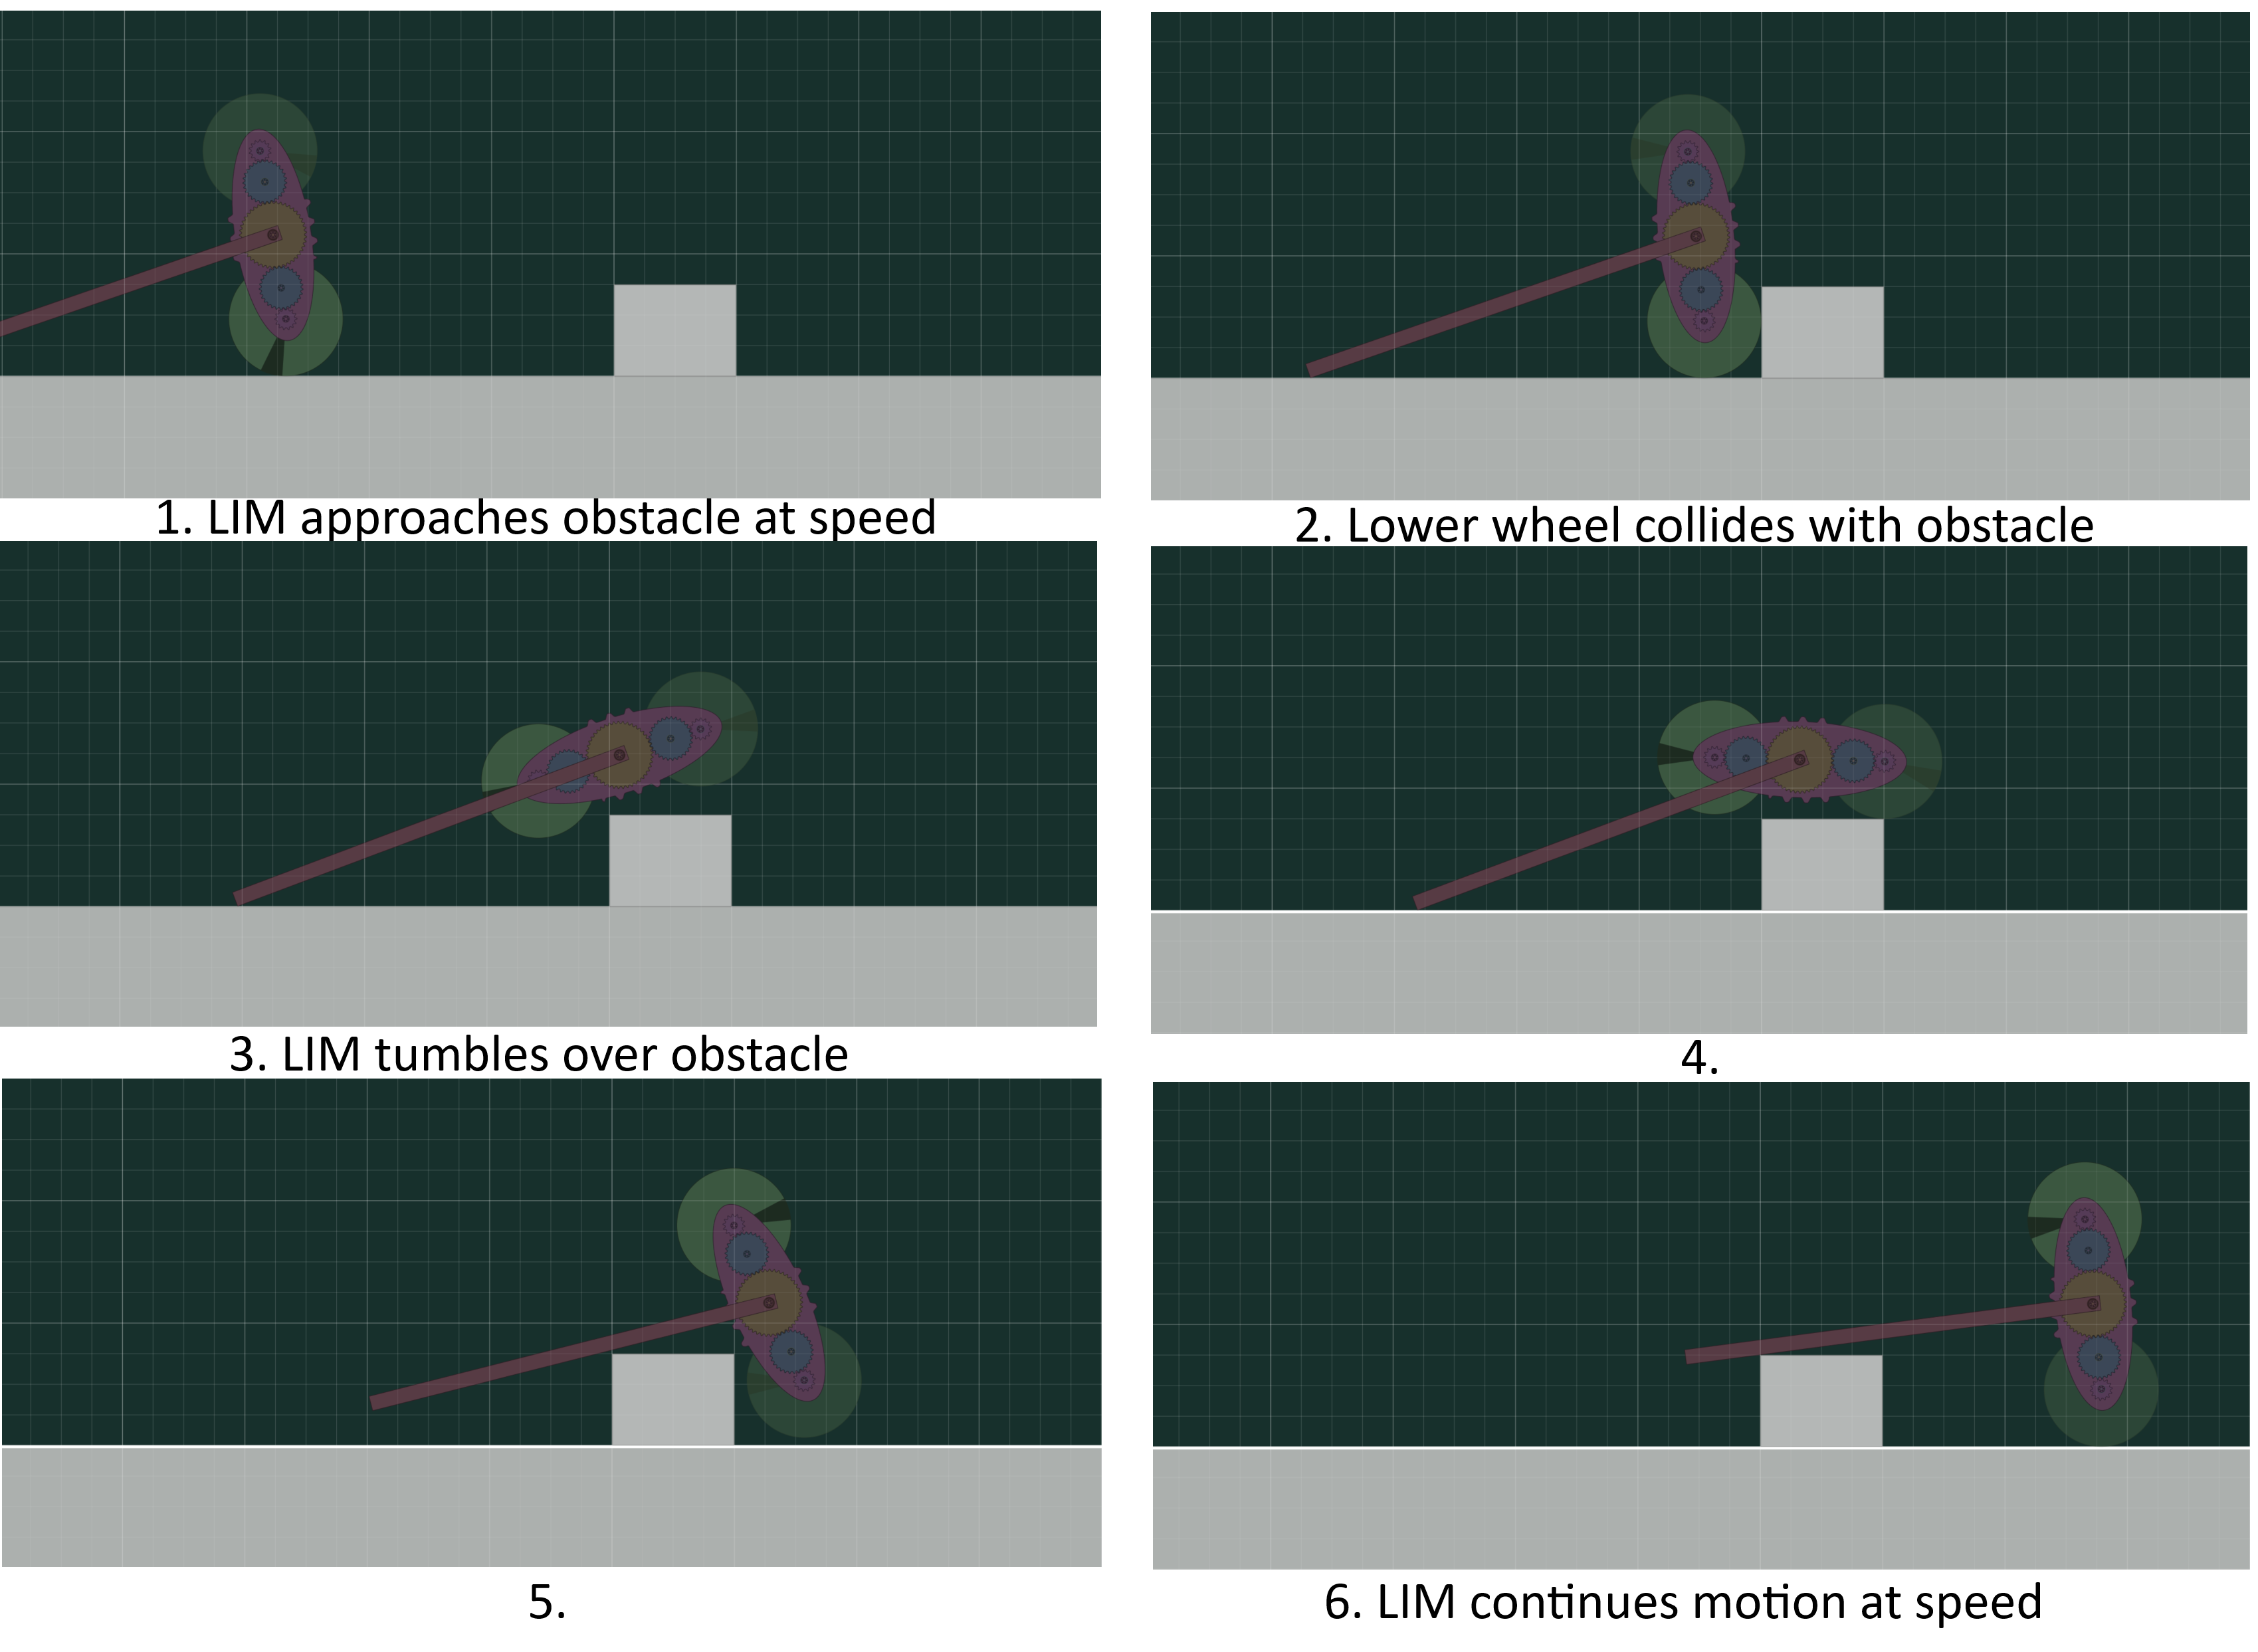
\includegraphics[width=1\textwidth]{algo-vert}
	\caption{Algodoo LIM system approaching obstacle vertically}
	\label{algo-vert}
\end{figure}

Another observation made was that if the LIM rolls at speed into the obstacle, it will have to absorb all the energy of the impact. None of the translational kinetic energy of the robot is transformed into rotational kinetic energy of the LIM for flipping. This results in quite an inefficient system. One option to mitigate this would be to implement a control system that solves the inverted pendulum problem in order to stand the LIMs upright on one wheel during normal operation. When the lower wheel encounters an obstacle while rolling, the LIM will readily flip over it without having to stop. The LIM could then switch to horizontal rolling when the robot needs a lower profile to enter a void. This solution would only be effective if a robust control system can be developed. These approaches are shown in Figures \ref{algo-hori} and \ref{algo-vert}.
\chapter{Design requirements}

The objective of the design phase is to design a LIMed platform that can be used to validate the mathematical model. The requirements for this design are documented in this section.

\section{Stakeholder requirements}

This project is done at the request of Justin Pead, who supervised previous LIM projects at UCT. For the purposes of this section, this project's supervisor, Mr. Wayne Swart, acts as an intermediary between the stakeholder and the designer. 


\begin{table}[h]
	\caption{Stakeholder requirements.}
	\footnotesize
	\begin{tabular}{ | p{3em} | p{6em} | p{23em} | p{5em} |} 
		\hline
		Number& Stakeholder & Description & Priority \\ 
		\hline
		SR1 & Justin Pead & The device must be able to climb stairs & High\\
		\hline
		SR2 & Justin Pead & The device must roll on its wheels when it is not obstructed, and climb over obstacles when it is obstructed. & High\\
		\hline
		SR3 & Justin Pead & The device must use LIMs for locomotion & Must-have\\
		\hline
		SR4 & Justin Pead & The device should be described by the model & Must have\\
		\hline
		SR5 & Justin Pead & The device should be relevant to USAR applications & High\\
		\hline
		SR6 & Wayne Swart & The design and construction of the device must demonstrate the relevant graduate attributes & Must have\\
		\hline
		SR7 & Wayne Swart & The budget for the project is R5000 & Must have\\
		\hline
	\end{tabular}
\end{table}
\newpage

\section{Engineering requirements}

In this section, the stakeholder requirements (SRs) are expressed as functional requirements (FRs) and performance requirements (PRs). FRs describe the actions that the system must perform, while PRs are measures of how well the system performs the functions.

\begin{table}[h]
	\caption{Functional requirements.}
	\footnotesize
	\begin{tabular}{ | p{4em} | p{28em} | p{6em} |} 
		\hline
		Number & Description & Relevant Stakeholder Requirement\\
		\hline
		FR1 & Climb obstacles & SR1, SR2\\
		\hline
		FR2 & Roll & SR2\\
		\hline
		FR3 & Accept user control & SR5\\
		\hline
	\end{tabular}
\end{table}

\begin{table}[h]
	\caption{Performance requirements.}
	\footnotesize
	\begin{tabular}{ 	| p{4em} 	| p{13em} 		| p{4em} 	| p{4em} 	| p{2em} 	| p{6em} |} 
		\hline
						Number & 	Description & 	Target & 	Range & 	Unit & 		Relevant Stakeholder Requirement\\
		\hline
		PR1 & Height of obstacles that can be climbed & Maximise & 200+ \tablefootnote{Maximum step rise specified by the SANS10400 building regulation \citep{SANS}} & mm &  SR1, SR2\\
		\hline
		PR2 & Climbing success rate & Maximise & 90 - 100 & \% &  SR1, SR2\\
		\hline
		PR3 & Top speed & Maximise & 1+ & $m/s$ &  SR2\\
		\hline
		PR4 & Acceleration & Maximise & 1+ & $m/s^2$ &  SR2\\
		\hline
		PR5 & Height Clearance & Minimise & 50 - 300 & $mm$ &  SR5\\
		\hline
		PR6 & Cost & Minimise & 0 - 5000 & ZAR &  SR6\\
		\hline
	\end{tabular}
\end{table}


\chapter{Design- 1st iteration}

Starting with Powrie's device as it is the most developed of the previous projects.\\
Attempted to use mathematical model to identify potential improvements, however I struggled to get objective improvements, increasing one parameter often may improve the ability to flip but hinder the ability to climb overall, and removing material should only be done if it has minimal effect on structure strength, something that would take much time to determine (possibly with FEM?). Such optimisations are beyond the scope of the project, I'm not trying to create a perfectly optimised device, I'm trying to create a working device so I can describe its function. Powrie’s device is working to some extent, so the first design iteration should deviate minimally from his design.\\
Powrie's design for the LIMs is copied as accurately as possible, could possibly even use his laser cutting templates to manufacture. Fortunately he provides a detailed builder's guide, allowing me to design and build ASAP so I can focus on the math model. The robot body is changed significantly. Powrie uses external gears on an already geared motor, this is unnecessary, as geared motors come in a variety of ratios. I use a JGY-370 motor, as I believe the worm gearbox is well suited to this purpose, it allows me to make a thinner body that doesn't protrude as far forward beyond the axle. The tail is designed based on Powrie’s concepts. The motors selected produce more torque than the ones Powrie selected, even with his additional gearing, so they should be up to the task. Later iterations could combine the worm gearbox with even more powerful brushless motors.
%\chapter{Conclusions}

This report details the design, modelling, and model validation of a novel gearing system for robot locomotion. The advantage of this LIM gearing system is that it allows a device to roll forward or climb steps using a single actuator, reducing costs, while also being able to fit into low voids. The model produced by this report could be used to inform the design of future USAR robots. This project builds and improves upon previous work, and produces the first LIM robot capable of climbing steps consistently and sequentially. \\

To explore the motion of the LIMS, a preliminary two-dimensional simulation was performed, and the stair climbing motion of the device was categorised into six distinct stages. This project proposes a mathematical model to describe the motion a LIMed device, using the MATLAB symbolic toolbox. The maths model consists of a large set of simultaneous equations that are solved simultaneously, and this report presents an algorithm that uses the MATLAB functions to efficiently solve this large set of equations. Additionally, this project explores the use of Drake, a multi-body simulator, to model the device. \\

Both the maths model and simulation are validated against real world data. The validation showed that the torque required to climb stairs sequentially was 16.4\% higher than the maths model predicted, and 5.9\% higher than the simulation predicted. This report explores the reasons for this error, which are attributed to incorrect assumptions and calibration methods.\\

In conclusion, this project was successful in completing its objectives. Both the model and simulation have been validated and their error has been quantified, they can be used to inform future work on LIMed robots.

\appendix%------------------------------------------------------------
\chapter{ECSA Outcome Self Assessment}

\begin{table}[h]
	\caption{ECSA outcome self assessment}
	\footnotesize
	\begin{tabular}{ | p{22em} | p{17em} |} 
		\hline
		ECSA outcome& Application \\ 
		\hline
		Demonstrate competence to identify, assess, formulate and solve convergent and
		divergent engineering problems creatively and innovatively. & 
		The design aspect of this project required creative solutions to overcome the limitations of previous designs. \\ 
		\hline
		Application of scientific and engineering knowledge: Demonstrate competence to apply knowledge
		of mathematics, basic science and engineering sciences from first principles to solve engineering problems. & 
		Producing the mathematical model required building a set of equations from first principles. \\ 
		\hline
		Engineering Design: Demonstrate competence to perform creative, procedural and non-procedural design and synthesis of components, systems, engineering works, products or processes.& This project designs a device, a model, a simulation pipeline, and an experiment. \\ 
		\hline
		Engineering methods, skills and tools, including Information Technology: Demonstrate competence
		to use appropriate engineering methods, skills and tools, including those based on information technology. & 
		The project involves designing a device using CAD, a controller in C, a math model in MATLAB, and a simulation pipeline using python.\\ 
		\hline
		Professional and technical communication: Demonstrate competence to communicate effectively,
		both orally and in writing, with engineering audiences and the community at large. & 
		All deliverables, including the proposal, progress report, final report, and presentation will demonstrate competent and effective communication. \\ 
		\hline
		Individual, Team and Multidisciplinary Working: Demonstrate competence to work effectively as an
		individual, in teams and in multi-disciplinary environments. & 
		This project is done individually, with input from the project supervisor and stakeholder. \\ 
		\hline
		Independent Learning Ability: Demonstrate competence to engage in independent learning through
		well-developed learning skills. & 
		Research is done in the literature review, and the use of tools such as Drake required independent learning. \\ 
		\hline
	\end{tabular}
\end{table}
\chapter{Mathematical proofs}

\section{Euler's equation}

\section{Navier Stokes equation}

\chapter{Experiment}

In order to validate that the model is accurate for each motion, the torque that causes the device to perform each motion determined experimentally. The equivalent values produced by the model can be compared with the measured torques to validate the model quantitatively. However, the torque produced by a DC motor cannot be measured or set directly. The torque of a DC motor is proportional to the current running through it, and when the motor isn't moving, the current is proportional to the voltage across the motor terminals. The terminal voltage is varied in this experiment.

\section{Voltage-torque calibration}
The relationship between terminal voltage and stalling torque is determined experimentally, this will allow subsequent experiments to measure the terminal voltage and calculate the stalling torque.
To characterise the motors, an experiment was set up to determine the stalling torque produced at different input voltages. In this experiment, a the motor lifts a lever with a mass attached. The torque required to lift the lever increases as the lever angle increases, until the motor can no longer provide enough torque and stalls. The lever angle which causes the motor to stall can be used to calculate the stalling torque, specifically by using the horizontal displacement of the mass,
\begin{equation}
	T_{Stall} = m g s_x
\end{equation}
where $T_{Stall}$ is the stalling torque, $m$ is the mass attached to the lever, $g$ is the gravitational acceleration, and $s_x$ is the horizontal displacement between the mass and the motor axis.
%figure here ????
This test is repeated with different motor voltages.\\

\subsection{Variables}
Independent variable:\\
$\bullet$ Motor voltage (V)\\
Dependent variable:\\
$\bullet$ Distance the weight is lifted (mm)\\
Controlled variables:\\
$\bullet$ Motor used\\
$\bullet$ Lever used\\
$\bullet$ Power supply used\\
$\bullet$ Multimeter used\\
$\bullet$ Ruler used\\

\subsection{Method}

\begin{enumerate}
	\item Remove LIM from motor axle.
	\item Attach the lever to the motor axle.
	\item Measure the weight of the mass on a calibrated scale. \label{stepMeasure}
	\item Drive the motor until the lever is pointing straight down.
	\item Attach the mass to the lever.
	\item Adjust the voltage of the power supply to the chosen value. \label{stepAdjust}
	\item Power on the motor.
	\item Wait until the lever stops moving.
	\item Record the voltage across the motor terminals. 
	\item Quickly power off the motor. Leaving the motor on while stalling can cause damage to the motor.
	\item Measure the horizontal distance that the lever has moved.
	\item Drive the motor until the lever is pointing straight down. \label{stepReset}
	\item Repeat steps \ref{stepAdjust} to \ref{stepReset} with different power supply voltages.
	\item Remove the mass from the lever. \label{stepRemove}
	\item Repeat steps \ref{stepMeasure} to \ref{stepRemove} with different masses.
\end{enumerate}
\subsection{Results}
The measured results, as well as the calculated torque, are shown in Table \ref{voltage-torque-table}, and visualised in Figure \ref{torque-voltage-plot}.

\begin{table}[!ht]
	\label{voltage-torque-table}
	\centering
	\begin{tabular}{|l|l|l|l|}
		\hline
		Mass (g) & Lever (mm) & Voltage (V) & Torque (Nm) \\ \hline
		145 & 97 & 0.83 & 0.13797765 \\ \hline
		145 & 101 & 0.92 & 0.14366745 \\ \hline
		145 & 151 & 1.1 & 0.21478995 \\ \hline
		204 & 154 & 1.22 & 0.30819096 \\ \hline
		204 & 229 & 1.56 & 0.45828396 \\ \hline
		542 & 89 & 1.72 & 0.47321478 \\ \hline
		537 & 106 & 1.93 & 0.55840482 \\ \hline
		542 & 106 & 1.8 & 0.56360412 \\ \hline
		537 & 164 & 2.45 & 0.86394708 \\ \hline
		542 & 171 & 2.5 & 0.90921042 \\ \hline
		542 & 220 & 3 & 1.1697444 \\ \hline
		542 & 242 & 3.25 & 1.28671884 \\ \hline
		1289 & 117 & 3.5 & 1.47947553 \\ \hline
		1289 & 136 & 4 & 1.71973224 \\ \hline
		1289 & 160 & 4.5 & 2.0232144 \\ \hline
	\end{tabular}
\end{table}

\begin{figure}[!h]
	\centering
	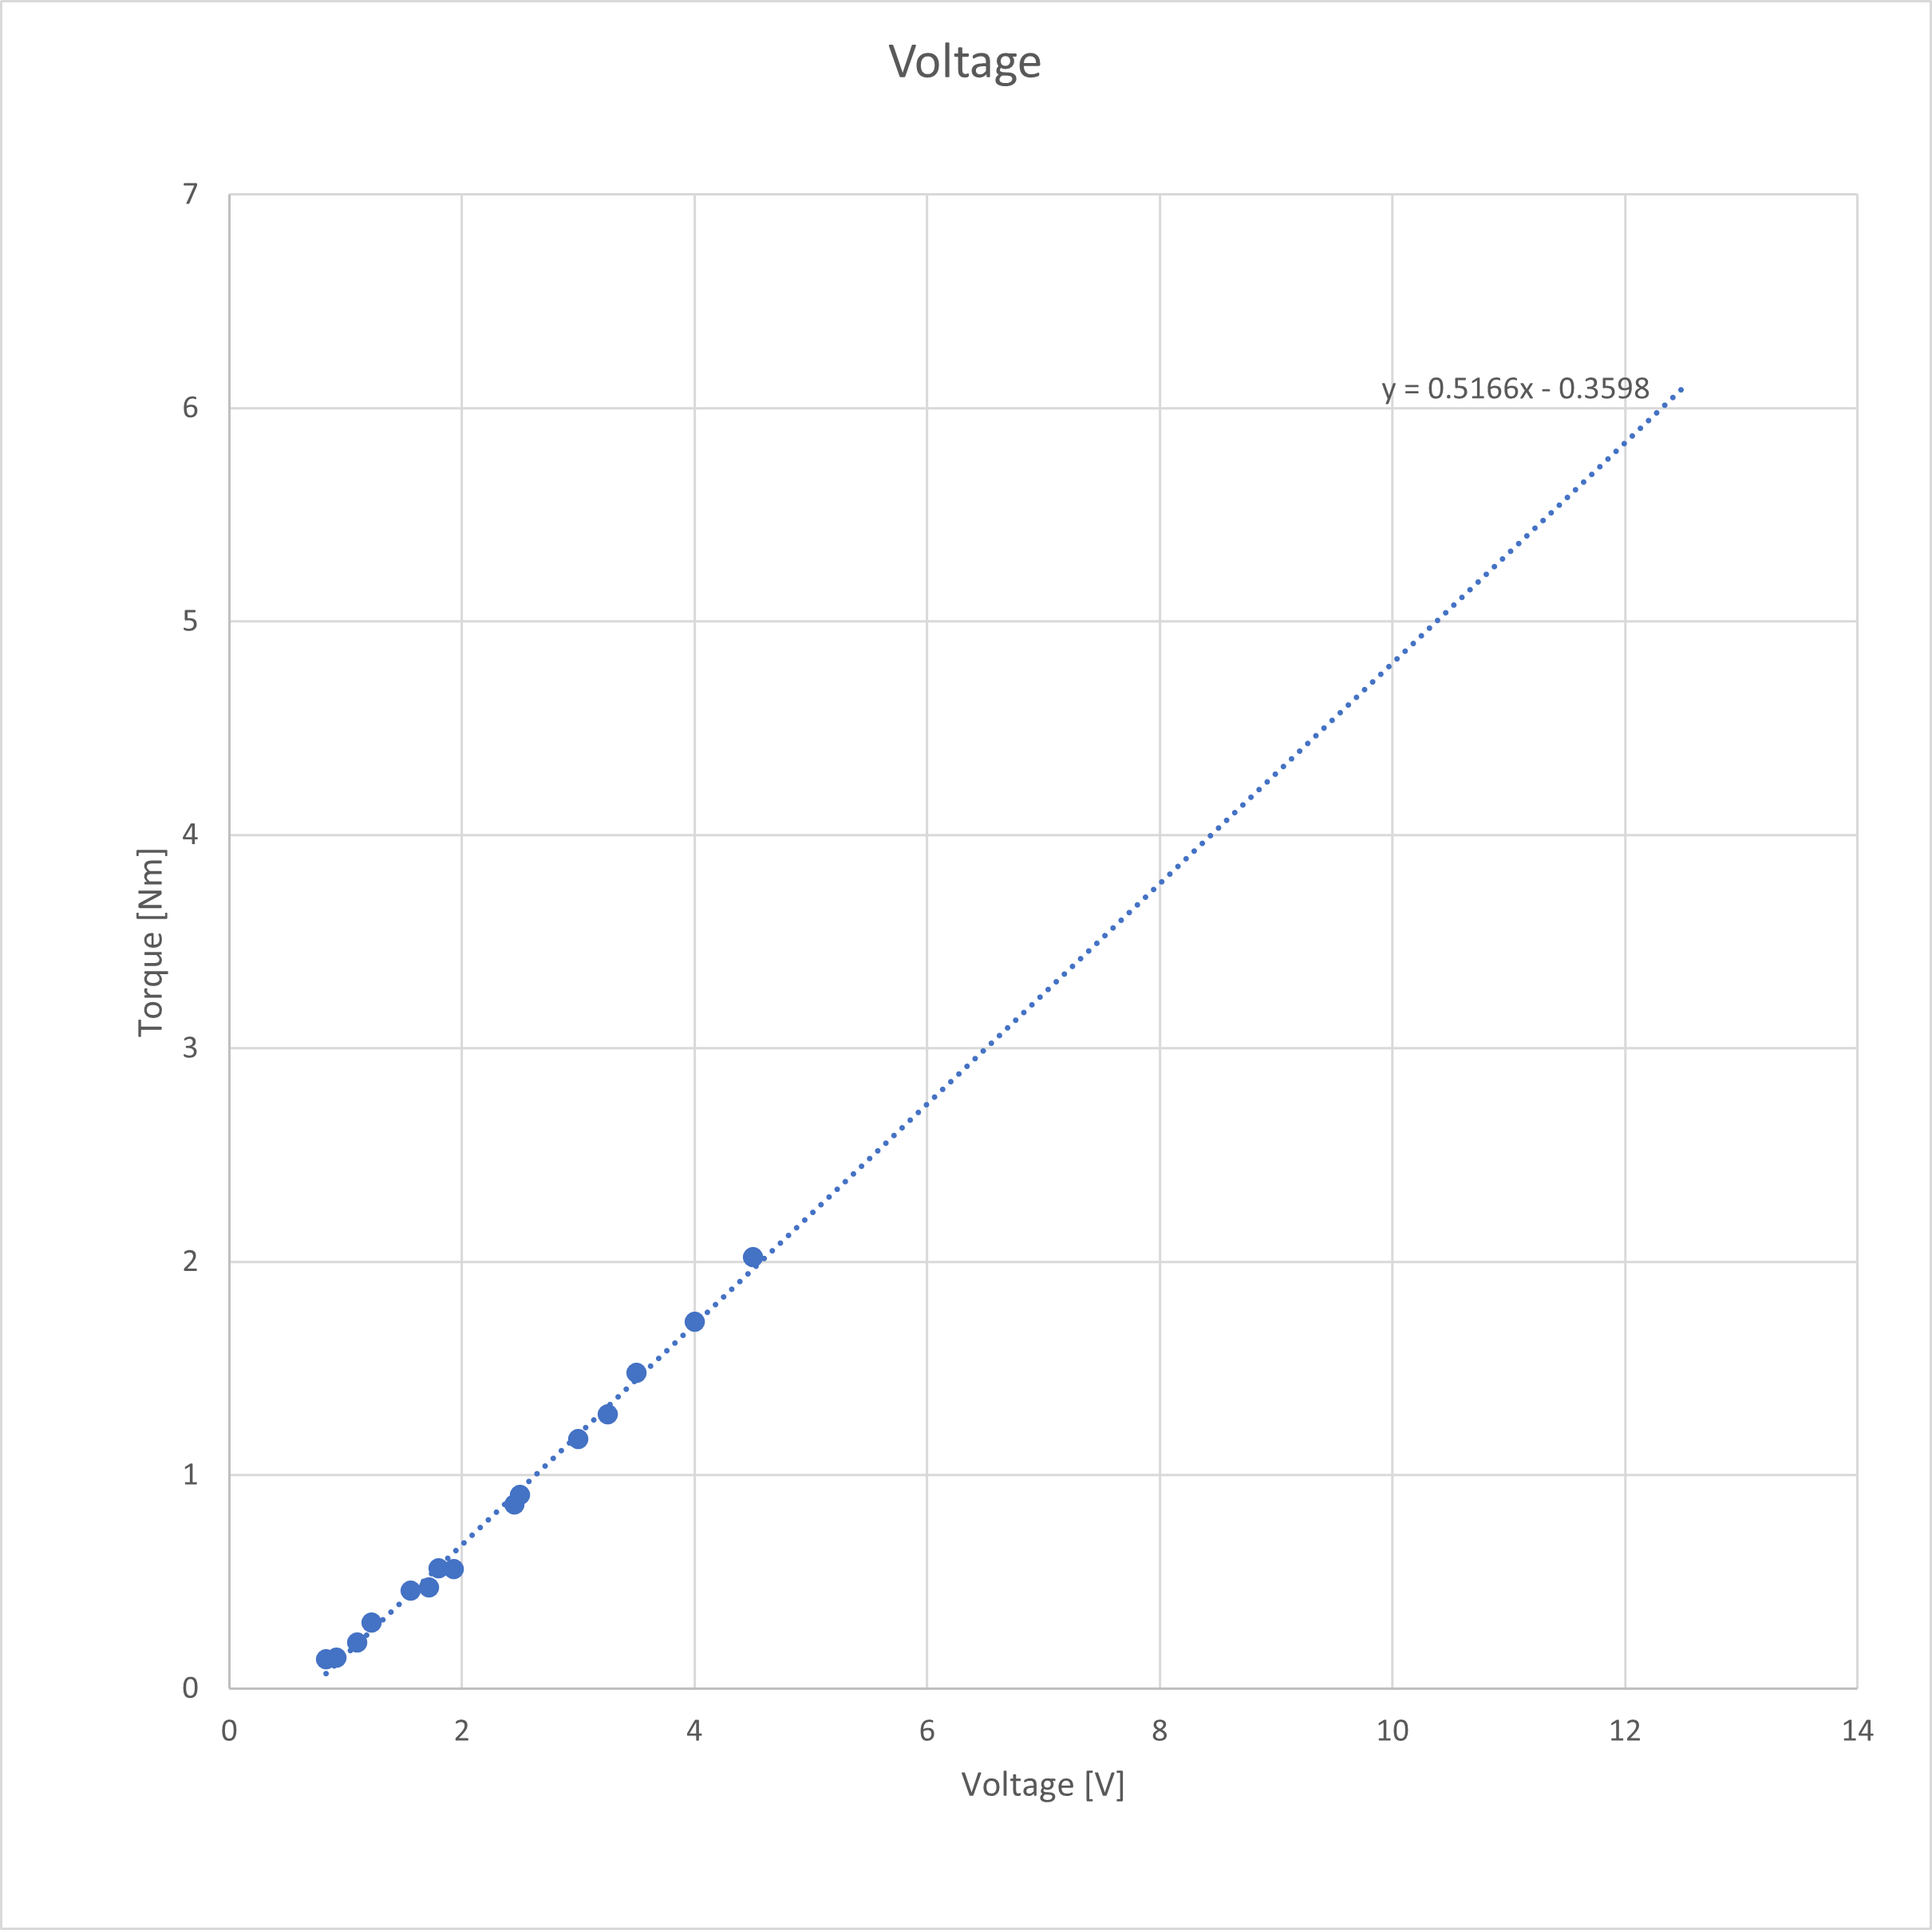
\includegraphics[width=0.8\textwidth]{plots/torque-voltage-relation.png}
	\caption{Relationship between motor voltage and stalling torque.}
	\label{torque-voltage-plot}
\end{figure}

This plot shows a linear relationship between stalling torque and voltage, and gives the formula,
\begin{equation}
	T_{Stall} =  0.5166 V - 0.3598 \label{eqTorqueVoltage}
\end{equation}
where $V$ is the motor terminal voltage.
This experiment did not attempt to measure torques beyond $2 Nm$ as this risked damaging the device and was beyond the expected requirements for the device.



\section{Climbing torque}
This experiment aims to determine the torque required to lift the device through each stage of motion. The results of this experiment will be compared with the compared with the theoretical torques required provided by the model and the simulation. The device is placed in the starting position for each stage of motion and powered with a certain supply voltage. The motion of the device is then assessed, if the device does not move then it is marked as "None"; if the device starts to move but does not complete the stage of motion, it is marked as "Partial"; and if it completes the stage of motion, it is marked as "Full".\\

%???? figure here

\subsection{Variables}
Independent variable:\\
$\bullet$ Motor voltage (V)\\
Dependent variable:\\
$\bullet$ Assessment of motion ("Full", "Partial", or "None")\\
Controlled variables:\\
$\bullet$ LIMed device\\
$\bullet$ Stairs\\
$\bullet$ Multimeter used\\


\subsection{Method}

\begin{enumerate}
	\item Place device in the starting position for the chosen stage of motion. \label{stepPlace}
	\item Adjust the voltage of the power supply to the chosen value.
	\item Power on the device.
	\item Observe how the device moves and classify the movement into "Full", "Partial", or "None". 
	\item Record the voltage across the motor terminals. 
	\item Power off the device.\label{stepOff}
	\item Repeat steps \ref{stepPlace} to \ref{stepOff} with a range of power supply voltages.\label{stepRepeatVoltage}
	\item Repeat steps \ref{stepPlace} to \ref{stepRepeatVoltage} for the different stages of motion.
\end{enumerate}

\subsection{Results}

Table \ref{tableStage1Torque} shows the measured results for the Stage 1 motion, as well as the torques calculated using Equation \ref{eqTorqueVoltage}. The data for the other stages of motion can be found in Appendix ???.

\begin{table}[!h]
	\caption{Torque experiment results for Stage 1}
	\label{tableStage1Torque}
	\centering
	\begin{tabular}{|l|l|l|}
		\hline
		Voltage (V) & Assessment of motion & Torque (Nm) \\ \hline
		0.89 & None & 0.099974 \\ \hline
		1.08 & None & 0.198128 \\ \hline
		1.12 & None & 0.218792 \\ \hline
		1.57 & None & 0.451262 \\ \hline
		1.68 & None & 0.508088 \\ \hline
		1.74 & None & 0.539084 \\ \hline
		1.81 & None & 0.575246 \\ \hline
		1.87 & None & 0.606242 \\ \hline
		1.89 & Partial & 0.616574 \\ \hline
		1.98 & Partial & 0.663068 \\ \hline
		2.05 & Partial & 0.69923 \\ \hline
		2.11 & Full & 0.730226 \\ \hline
		2.13 & Full & 0.740558 \\ \hline
		2.25 & Full & 0.80255 \\ \hline
		2.26 & Full & 0.807716 \\ \hline
		2.3 & Full & 0.82838 \\ \hline
	\end{tabular}
\end{table}

This data is plotted in Figure \ref{plotassessment-torque-relation-stage1}, which shows that the full motion only happens with torques of at least $0.73 Nm$, while partial motion only requires $0.61 Nm$.

\begin{figure}[h]
	\centering
	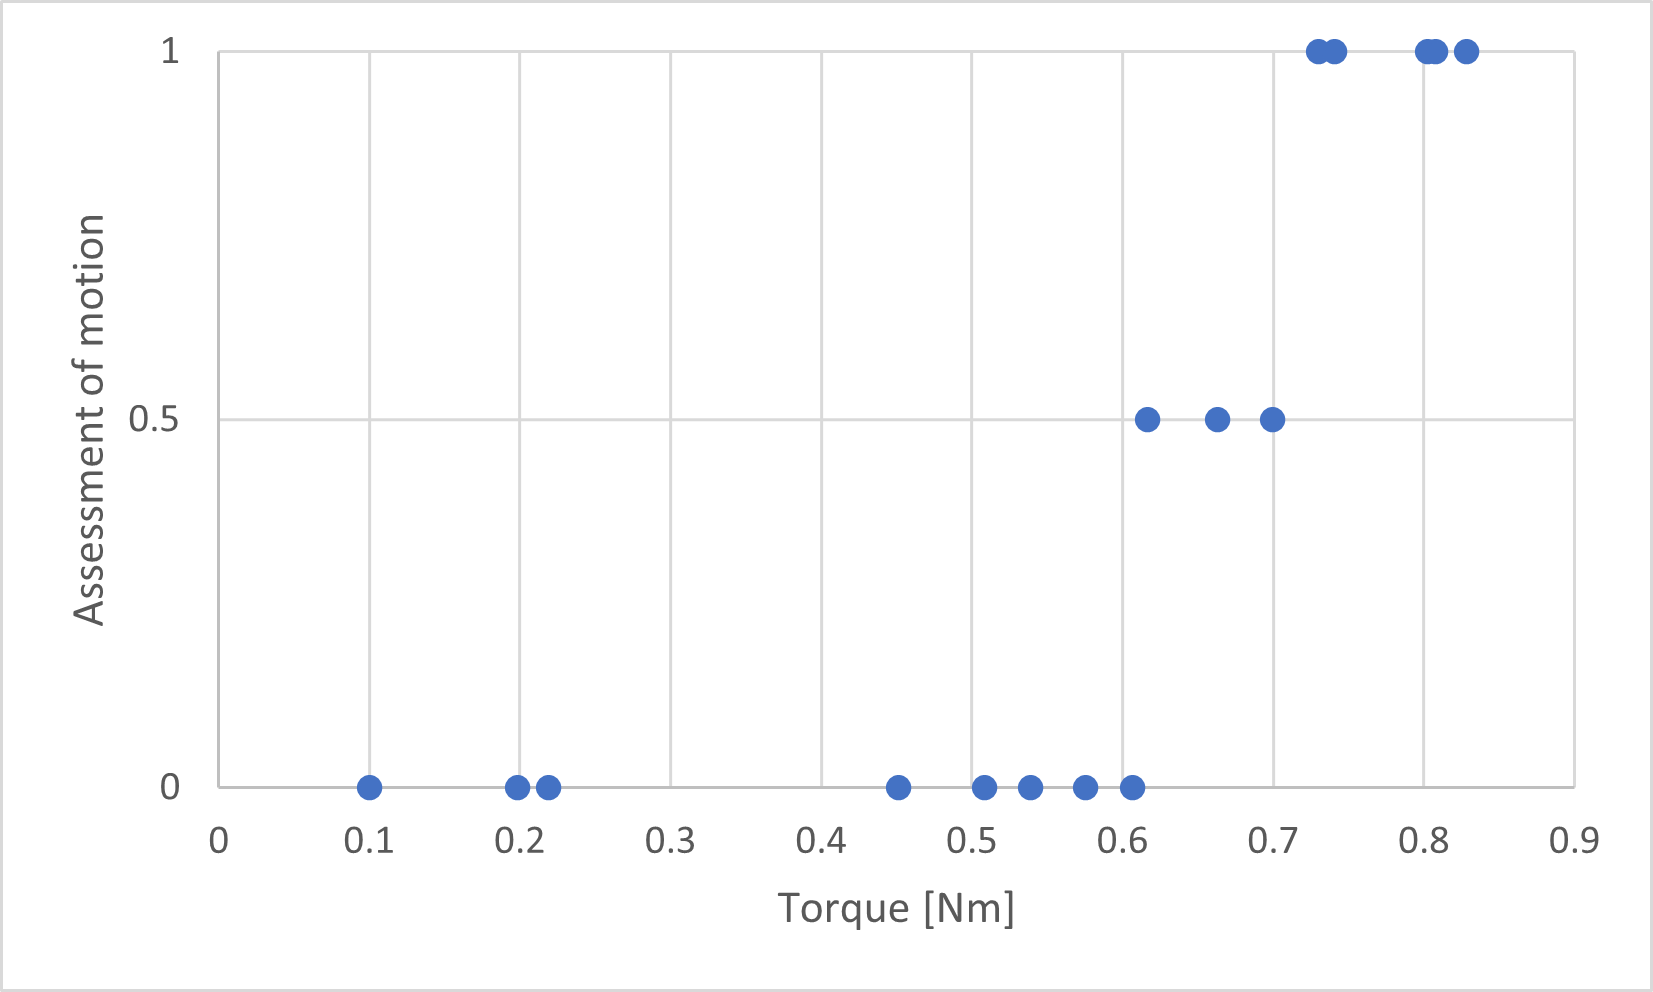
\includegraphics[width=0.8\textwidth]{plots/assessment-torque-relation-stage1}
	\caption{Relationship between torque and motion for Stage 1, with 0, 0.5, and 1 representing "None", "Partial", and "Full" respectively.}
	\label{plotassessment-torque-relation-stage1}
\end{figure}




\backmatter%----------------------------------------------------------
\bibliography{bib/bib-sample}
 
\end{document}   

